% Options for packages loaded elsewhere
\PassOptionsToPackage{unicode}{hyperref}
\PassOptionsToPackage{hyphens}{url}
\PassOptionsToPackage{dvipsnames,svgnames*,x11names*}{xcolor}
%
\documentclass[
  11pt,
]{article}
\usepackage[]{mathpazo}
\usepackage{amsmath}
\usepackage{ifxetex,ifluatex}
\ifnum 0\ifxetex 1\fi\ifluatex 1\fi=0 % if pdftex
  \usepackage[T1]{fontenc}
  \usepackage[utf8]{inputenc}
  \usepackage{textcomp} % provide euro and other symbols
  \usepackage{amssymb}
\else % if luatex or xetex
  \usepackage{unicode-math}
  \defaultfontfeatures{Scale=MatchLowercase}
  \defaultfontfeatures[\rmfamily]{Ligatures=TeX,Scale=1}
\fi
% Use upquote if available, for straight quotes in verbatim environments
\IfFileExists{upquote.sty}{\usepackage{upquote}}{}
\IfFileExists{microtype.sty}{% use microtype if available
  \usepackage[]{microtype}
  \UseMicrotypeSet[protrusion]{basicmath} % disable protrusion for tt fonts
}{}
\usepackage{xcolor}
\IfFileExists{xurl.sty}{\usepackage{xurl}}{} % add URL line breaks if available
\IfFileExists{bookmark.sty}{\usepackage{bookmark}}{\usepackage{hyperref}}
\hypersetup{
  pdftitle={Making Migration Sexy: How State and National Policies Influence Migration of Same-Sex Couples},
  pdfauthor={Nathan I. Hoffmann, Department of Sociology, University of California, Los Angeles; Kristopher Velasco, Department of Sociology, University of Texas at Austin},
  pdfkeywords={immigration, same-sex couples, LGBTQ policy, sexuality},
  colorlinks=true,
  linkcolor=blue,
  filecolor=Maroon,
  citecolor=Blue,
  urlcolor=Blue,
  pdfcreator={LaTeX via pandoc}}
\urlstyle{same} % disable monospaced font for URLs
\usepackage[margin=1in]{geometry}
\usepackage{longtable,booktabs}
\usepackage{calc} % for calculating minipage widths
% Correct order of tables after \paragraph or \subparagraph
\usepackage{etoolbox}
\makeatletter
\patchcmd\longtable{\par}{\if@noskipsec\mbox{}\fi\par}{}{}
\makeatother
% Allow footnotes in longtable head/foot
\IfFileExists{footnotehyper.sty}{\usepackage{footnotehyper}}{\usepackage{footnote}}
\makesavenoteenv{longtable}
\usepackage{graphicx}
\makeatletter
\def\maxwidth{\ifdim\Gin@nat@width>\linewidth\linewidth\else\Gin@nat@width\fi}
\def\maxheight{\ifdim\Gin@nat@height>\textheight\textheight\else\Gin@nat@height\fi}
\makeatother
% Scale images if necessary, so that they will not overflow the page
% margins by default, and it is still possible to overwrite the defaults
% using explicit options in \includegraphics[width, height, ...]{}
\setkeys{Gin}{width=\maxwidth,height=\maxheight,keepaspectratio}
% Set default figure placement to htbp
\makeatletter
\def\fps@figure{htbp}
\makeatother
\setlength{\emergencystretch}{3em} % prevent overfull lines
\providecommand{\tightlist}{%
  \setlength{\itemsep}{0pt}\setlength{\parskip}{0pt}}
\setcounter{secnumdepth}{5}
\usepackage{fancyhdr}
\pagestyle{fancy}
\setlength{\headheight}{13.6pt}
\rhead{\textit{Hoffmann and Velasco}}
\lhead{\textit{April 11, 2021}}
\usepackage{booktabs}
\usepackage{longtable}
\usepackage{array}
\usepackage{multirow}
\usepackage{wrapfig}
\usepackage{float}
\usepackage{colortbl}
\usepackage{pdflscape}
\usepackage{tabu}
\usepackage{threeparttable}
\usepackage{threeparttablex}
\usepackage[normalem]{ulem}
\usepackage{makecell}
\usepackage{xcolor}
\ifluatex
  \usepackage{selnolig}  % disable illegal ligatures
\fi
\newlength{\cslhangindent}
\setlength{\cslhangindent}{1.5em}
\newlength{\csllabelwidth}
\setlength{\csllabelwidth}{3em}
\newenvironment{CSLReferences}[2] % #1 hanging-ident, #2 entry spacing
 {% don't indent paragraphs
  \setlength{\parindent}{0pt}
  % turn on hanging indent if param 1 is 1
  \ifodd #1 \everypar{\setlength{\hangindent}{\cslhangindent}}\ignorespaces\fi
  % set entry spacing
  \ifnum #2 > 0
  \setlength{\parskip}{#2\baselineskip}
  \fi
 }%
 {}
\usepackage{calc}
\newcommand{\CSLBlock}[1]{#1\hfill\break}
\newcommand{\CSLLeftMargin}[1]{\parbox[t]{\csllabelwidth}{#1}}
\newcommand{\CSLRightInline}[1]{\parbox[t]{\linewidth - \csllabelwidth}{#1}\break}
\newcommand{\CSLIndent}[1]{\hspace{\cslhangindent}#1}

\title{Making Migration Sexy: How State and National Policies Influence Migration of Same-Sex Couples\thanks{The authors contributed equally to this paper.}}
\author{Nathan I. Hoffmann, Department of Sociology, University of California, Los Angeles \and Kristopher Velasco, Department of Sociology, University of Texas at Austin}
\date{April 11, 2021}

\begin{document}
\maketitle
\begin{abstract}
As same-sex couples gain greater social acceptance and new rights, their numbers reported on surveys are rapidly increasing in the United States. Yet few researchers have studied immigrants in same-sex couples on a large scale. Using the American Community Survey from 2008 to 2019, this study compares immigrants in same-sex couples to corresponding different-sex couples in order to characterize and assess the scale of ``sexual migration'' to the U.S. Moreover, we evaluate how the policy environment regarding same-sex couples shapes migratory patterns. Fixed effects models show that as origin countries become more LGBT-friendly, we see more LGB immigrants from those countries in the U.S. On the individual level, immigrants in same-sex couples are more likely to live in progressive U.S. states, an effect that increases in strength as migrants come from for more LGBT-friendly countries of origin. We also find that, compared to different-sex immigrant couples, immigrants in same-sex couples come from richer, more democratic countries that are less represented in immigrant networks. Our findings put into question dominant models of migration that emphasize economic and network effects, suggesting the importance of considering sexuality as well as political and lifestyle motivations more broadly.
\end{abstract}

\hypertarget{introduction}{%
\section{Introduction}\label{introduction}}

In 2013, the U.S. Supreme Court made a landmark decision overturning the Defense of Marriage Act, requiring the U.S. federal government to recognize marriages between same-sex spouses. This decision radically changed the immigration landscape for same-sex couples: For the first time, same-sex spouses of U.S. citizens and legal permanent residents were eligible file a spousal petition for an immigrant visa (\protect\hyperlink{ref-edwards_2013}{Edwards, 2013}). In the years since, the U.S. population of immigrants in same-sex couples has grown rapidly. While numbers of different-sex couples including immigrants increased by 13 percent from 2013 to 2019 (from 8.4 million to 9.5 million), those of corresponding same-sex couples grew from 61 thousand to 107 thousand in the same period, an increase of 76 percent (\protect\hyperlink{ref-ruggles_2021}{Ruggles et al., 2021}). Indeed, this time period represents an important moment in which policies governing same-sex couples, both in the U.S. and internationally, are changing rapidly. Although scholars have briefly described the lesbian, gay, and bisexual (LGB) immigrant population (\protect\hyperlink{ref-gates_2013}{Gates, 2013a}; \protect\hyperlink{ref-goldberg_2021}{Goldberg \& Conron, 2021}), immigration research has not explicitly analyzed how policy changes are influencing the migration patterns of individuals in same-sex couples into and across the U.S. This is partly due to the fact that conventional migration research has only recently begun to factor in the role of social policies not explicitly in the realm of immigration policy (\protect\hyperlink{ref-fitzgerald_2014}{Fitzgerald et al., 2014}). Moreover, while gender has been recently recognized as an integral part of the migration process (\protect\hyperlink{ref-hondagneu-sotelo_2012}{Hondagneu-Sotelo, 2012}; \protect\hyperlink{ref-lutz_2010}{Lutz, 2010}), sexuality has received scant attention. Recent qualitative work has demonstrated, however, that sexuality is a salient factor influencing migration decisions (\protect\hyperlink{ref-ahmad_2013}{Ahmad, 2013}; \protect\hyperlink{ref-carrillo_2018}{Carrillo, 2018}; \protect\hyperlink{ref-gorman-murray_2009}{Gorman-Murray, 2009}; \protect\hyperlink{ref-mai_2009}{Mai \& King, 2009}). We show that differences between immigrants in same-sex couples and those in different-sex couples cannot be explained solely using classic theories of migration; consequently, not making sexuality an integral part of the research question limits our understanding of the full migration process.

Therefore, we seek to understand how LGBT policies at country-of-origin and of U.S. state of residence influence migration patterns of immigrants in same-sex relationships. We integrate two types of data to help answer this question. First, we rely on American Community Survey (ACS) data for 2008 to 2019 (\protect\hyperlink{ref-ruggles_2021}{Ruggles et al., 2021}), which allows the identification of same-sex couples, immigrant origin, U.S. state of residence, and potentially confounding individual characteristics. Second, we harness original datasets indexing LGBT policy changes in 193 countries and all U.S. states from 1991 to 2019 (\protect\hyperlink{ref-velasco_2020}{Velasco, 2020}). We merge these two primary data sources with country- and state-level control variables from the UN, World Bank, U.S. government, and other sources.

Our analytic strategy proceeds in four parts. First, we descriptively try to understand who these same-sex couples are. This first step is important because little is known about this growing population. We contrast immigrants in same- and different-sex couples, assessing how classic migration variables such as wage differentials, individual income, and co-national networks compare between these groups. Second, we focus on country-of-origin effects, modeling how same-sex immigrant couple representation changes over time in relation to the LGBT policy context of the country of origin. Third, we factor in the role of changing state LGBT policy context in models at the U.S. state level. Lastly, we shift our attention to the individual, assessing how being an immigrant in a same-sex couple, net of other individual factors usually considered in migration analyses, bears upon choice of LGBT policy context by state. We also consider how this relationship is moderated by LGBT policy context in the country of origin.

Our research demonstrates that origin-country policies matter for levels of immigrants in same-sex couples, but perhaps not in the way expected. Countries of origin with more LGBT-friendly policies send higher proportions of immigrants in same-sex couples. This implies that these policies may enable the migration aspirations of LGBT individuals, whereas oppressive policies may hinder such ambitions. Second, we find little role of U.S. state policy at the aggregate level of proportion immigrants in same-sex couples. But at the individual level, we find the expected trend: Immigrants in same-sex couples are more likely to live in LGBT-friendly states. This effect is moderated by country-of-origin context, however; immigrants in same-sex couples from countries with LGBT-friendly policies are more likely to live in LGBT-friendly states. We find the opposite trend for immigrants in different-sex couples. The findings from this project highlight how the interaction between sexuality and political context shape migration decisions, underscoring the importance of considering political and ``lifestyle'' variables in the migration process (\protect\hyperlink{ref-benson_2012}{Benson \& O'Reilly, 2012}; \protect\hyperlink{ref-fitzgerald_2014}{Fitzgerald et al., 2014}).

\hypertarget{background-changing-policy-landscape-for-same-sex-immigrant-couples}{%
\section{Background: Changing Policy Landscape for Same-Sex Immigrant Couples}\label{background-changing-policy-landscape-for-same-sex-immigrant-couples}}

The U.S. has undergone significant shifts in the policies governing LGBT populations at both state and federal levels. Since 2003, the U.S. Supreme Court has ruled sodomy laws and the Defense of Marriage Act unconstitutional, recognized same-sex marriages at the federal level, and curtailed employment discrimination. In response, several U.S. states implemented new policies hindering LGBT communities on top of existing discriminatory policies like state constitutional bans on marriage equality (\protect\hyperlink{ref-kazyak_2018}{Kazyak et al., 2018}). These dynamics create a varied landscape in which state lines significantly demarcate the types of rights and legal environments LGBT people experience. Now, a burgeoning area of scholarship exists to understand the causes of these transformations (\protect\hyperlink{ref-lax_2009}{Lax \& Phillips, 2009}; \protect\hyperlink{ref-soule_2004}{Soule, 2004}) and their distinct consequences on the lives and well-being of LGBT people (\protect\hyperlink{ref-boertien_2019}{Boertien \& Vignoli, 2019}; \protect\hyperlink{ref-carpenter_2020}{Carpenter, 2020}; \protect\hyperlink{ref-kail_2015}{Kail et al., 2015}; \protect\hyperlink{ref-levy_2017}{Levy \& Levy, 2017}).

Though this changing policy landscape affects LGBT populations of all types, particular sub-groups within this broad umbrella are likely to be differentially impacted. Same-sex immigrant couples represent a key group especially vulnerable to recent changes. This is because prior to being able to experience recognized rights like marriage or non-discrimination protections, same-sex immigrant couples must first be able to enter into the U.S. Historically, federal U.S. law hindered same-sex immigrant couples' ability to enter the country due to the government's lack of recognition of their relationship (\protect\hyperlink{ref-humanrightswatch_2006}{Human Rights Watch, 2006}). One of the few mechanisms available to queer migrants for entering the U.S. was through asylum claims -- an invasive process in which migrants needed to ``prove'' their sexual desires and potential persecution (\protect\hyperlink{ref-humanrightswatch_2006}{Human Rights Watch, 2006}). These broad legal exclusions often carry over to academic scholarship as well. Analyses of domestic LGBT communities often assume citizenship and migration research presents migrants as heterosexual (\protect\hyperlink{ref-luibheid_2008}{Luibhéid, 2008}). The academic research that does acknowledge the realities of queer migrants, though, is largely centered on the asylum claims and offers a qualitative insight into how queer migrants navigate this process (\protect\hyperlink{ref-vogler_2016}{Vogler, 2016}). As such, there is presently a shallow understanding of the factors broadly influencing the migratory patterns of same-sex immigrant couples beyond this pathway and how these patterns align or diverge from their well-studied heterosexual counterparts. Indeed, even broad, descriptive understandings of migrants in same-sex relationships within the U.S. is absent within academic literature. This leaves a significant blindspot.

\begin{figure}
\centering
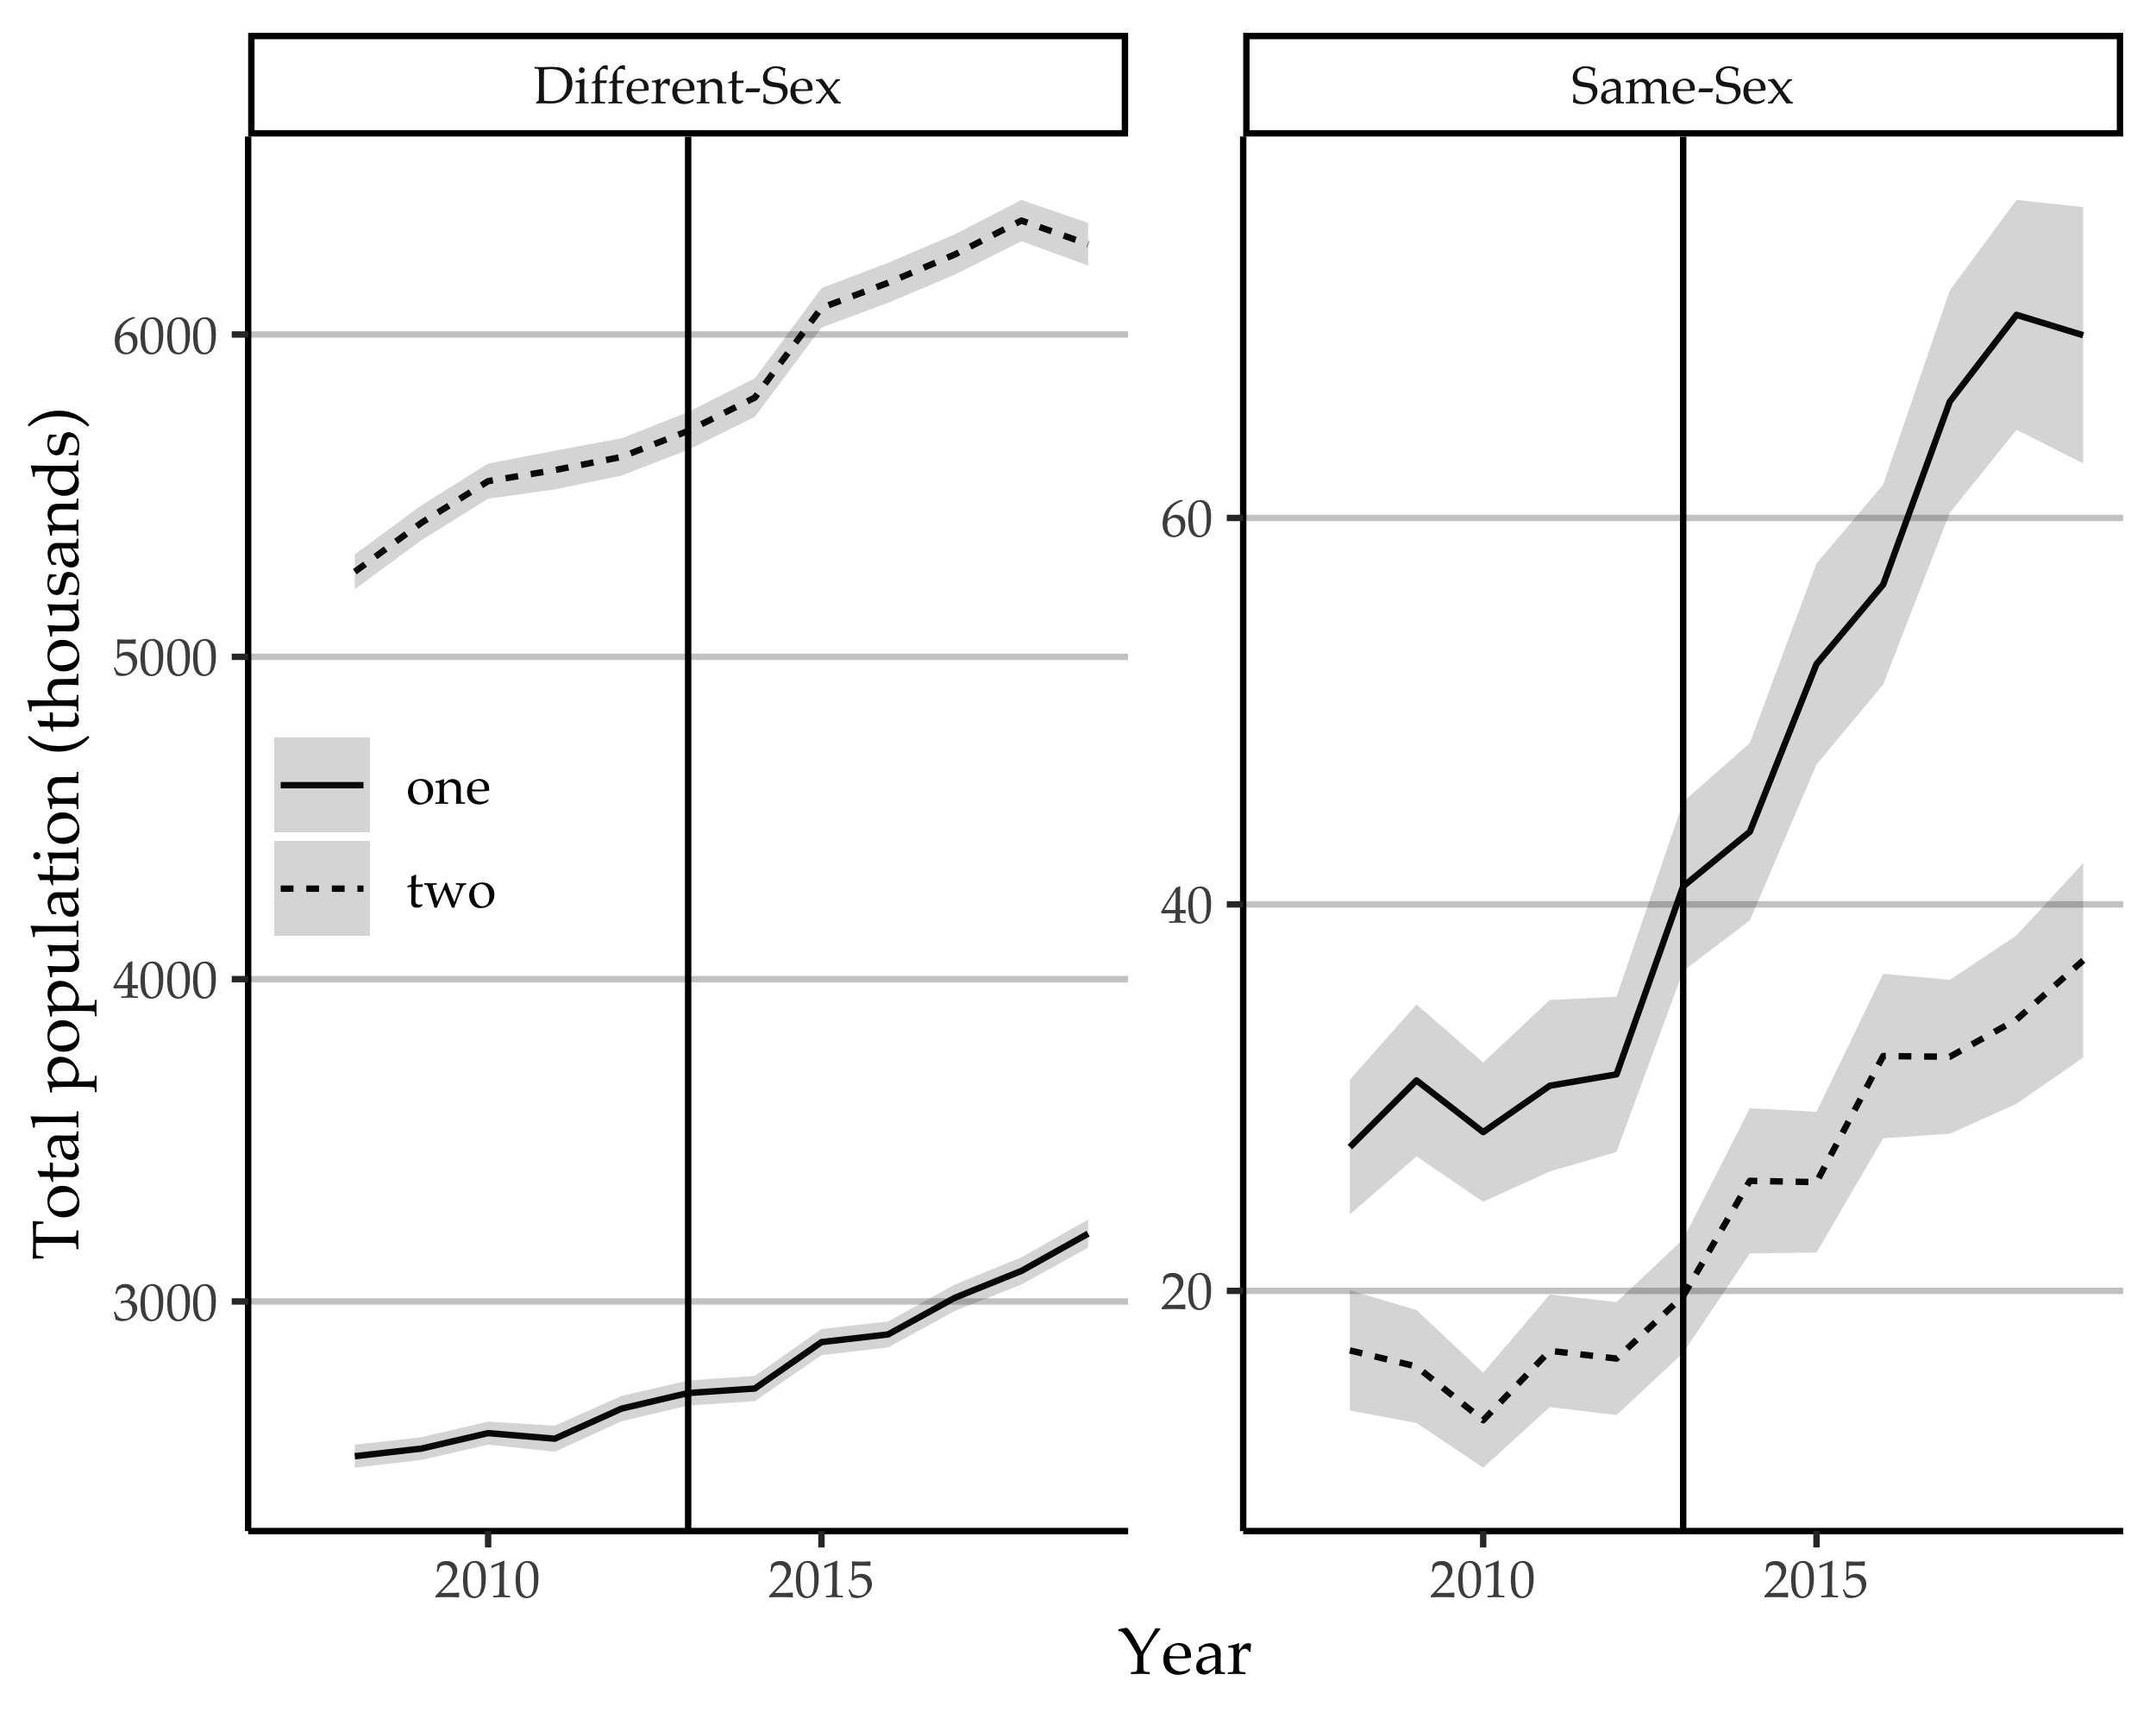
\includegraphics{ssimm_draft_files/figure-latex/total-pop-1.pdf}
\caption{\label{fig:total-pop}Estimated totals of different- and same-sex couples containing one or two immigrants, 2008-2019, with 95\% confidence intervals. Vertical line placed at the year 2013, when DOMA was overturned.}
\end{figure}

The federal environment governing immigration significantly changed after 2013. The U.S. Supreme Court opinion ruling the Defense of Marriage Act (DOMA) unconstitutional opened the door for more same-sex immigrant couples to enter the U.S. under the same process long-governing different-sex couples (\protect\hyperlink{ref-edwards_2013}{Edwards, 2013}). Indeed, as Figure \ref{fig:total-pop} highlights, the number of same-sex immigrant couples in the U.S. grew significantly following this ruling -- especially when compared to different-sex couples. Aside from allowing gay and lesbian families to remain unified, this national opening creates an important moment for the scholarly community as well. Now, more careful investigations into the factors both pushing and pulling same-sex immigrant couples into the U.S. can be conducted beyond idiosyncratic asylum claims. The present research fits squarely within this critical research gap.

\hypertarget{understanding-influences-on-migration-patterns}{%
\section{Understanding Influences on Migration Patterns}\label{understanding-influences-on-migration-patterns}}

\hypertarget{conventional-explanations}{%
\subsection{Conventional Explanations}\label{conventional-explanations}}

Our analysis compares conventional explanations for migration to political ones related to LGBT policy. Massey et al. (\protect\hyperlink{ref-massey_1999}{1999, p. 50}) provided an influential synthesis of migration theories from economics and sociology, arguing that ``causal processes relevant to international migration might operate on multiple levels simultaneously.'' Our investigation incorporates insights from their work as well as assesses how sexuality and LGBT policy complicate migration analysis. At one level, economic theories underscore that promise of material gain is a frequent motivation to migrate (\protect\hyperlink{ref-hatton_2005a}{Hatton \& Williamson, 2005}; \protect\hyperlink{ref-todaro_1980}{Todaro, 1980}), predicting that migrants will follow wage and unemployment differentials across countries. To account for migration costs, models often adjust for distance: Immigrants are more likely to migrate between proximate countries, especially those that share a border. At another level, migration streams often continue even after wage differentials decrease due to immigrant networks; migrants share information and resources to lower the cost of migration and settling in the destination country (\protect\hyperlink{ref-massey_1987}{Massey et al., 1987}). Quantitative scholars often measure immigration networks using the relative size of co-national immigrant stock (\protect\hyperlink{ref-beine_2016}{Beine et al., 2016}).

More recent sociological theories of migration add political and cultural variables to the causal mix (\protect\hyperlink{ref-fitzgerald_2014}{Fitzgerald et al., 2014}; \protect\hyperlink{ref-karemera_2000}{Karemera et al., 2000}; \protect\hyperlink{ref-mayda_2010}{Mayda, 2010}). Scholars have shown that shared language, colonial history, and democracy matter in the sending country, and immigrant rights matter in the receiving country. In this paper, we borrow terminology from economics and use the term ``gravity model'' to describe the combination of economic, network, and political variables into a single quantitative model to predict migration (\protect\hyperlink{ref-anderson_2011}{Anderson, 2011}; \protect\hyperlink{ref-beine_2016}{Beine et al., 2016}).

Previous scholarship has not explicitly applied these analyses and insights to the migration of same-sex couples on a large scale in the U.S. context. Consequently, we do not know how the theories of migration synthesized by \protect\hyperlink{ref-massey_1999}{Massey et al.} (\protect\hyperlink{ref-massey_1999}{1999}) hold for this subpopulation. Previous demographic research on non-immigrant same-sex couples suggest characteristics salient to the migration process may still relate to their migration. In the labor market, men in same-sex couples tend to earn less than their heterosexual counterparts, but women tend to earn more (\protect\hyperlink{ref-klawitter_2015}{Klawitter, 2015}). On average, married same-sex couples are older and have higher earnings than their different-sex counterparts (\protect\hyperlink{ref-fisher_2018}{Fisher et al., 2018}), while results for unmarried couples are mixed (\protect\hyperlink{ref-baumle_2009}{Baumle et al., 2009}). If immigrants in same-sex couples have higher earnings than heterosexual immigrants, then the typical economic push and pull factors of immigration may affect them differently. As discussed below, one difference is that these higher earnings may open pathways for lifestyle factors to influence their migration decisions (\protect\hyperlink{ref-benson_2009}{Benson \& O'Reilly, 2009}; \protect\hyperlink{ref-dixon_2020}{Dixon, 2020}). Same-sex couples also tend to be less homogamous in age, education, and race/ethnicity than their different-sex counterparts (\protect\hyperlink{ref-schwartz_2009}{Schwartz \& Graf, 2009}).

Sexuality may interact with processes of migration in ways not anticipated by the migration theories synthesized by \protect\hyperlink{ref-massey_1999}{Massey et al.} (\protect\hyperlink{ref-massey_1999}{1999}) or even recent work on political and cultural factors. We seek to intervene within migration scholarship by explicitly considering how sexuality, and the governance of it, expand our comprehension of migration atop this previous work.

\hypertarget{our-intervention}{%
\subsection{Our Intervention}\label{our-intervention}}

We argue that it is imperative to take sexuality, and the state's role in governing sexuality, into account for understanding migratory patterns (\protect\hyperlink{ref-cantu_2009}{Cantú, 2009}; \protect\hyperlink{ref-carrillo_2018}{Carrillo, 2018}). One reason why this area of research has yet to be fully considered, in addition to previous restrictions outlined, is because the literature largely assumes immigrants are heterosexual or simply neglects to consider them as fully constitutive, diverse sexual beings (\protect\hyperlink{ref-canaday_2009}{Canaday, 2009}; \protect\hyperlink{ref-epstein_2014}{Epstein \& Carrillo, 2014}; \protect\hyperlink{ref-gonzalez-lopez_2005}{González-López, 2005}).

Consequently, analyses into how sexuality motivates migratory decisions or how migration reimagines sexual behaviors and understandings are limited (\protect\hyperlink{ref-carrillo_2018}{Carrillo, 2018}). Even more limited are explicit analyses into how policies such as same-sex marriage, hate crime protections, sodomy, and the like, further influence migration patterns. The nascent scholarship concerning queer migrants that does exist, though, suggests that policy environments are a central concern when making these decisions (\protect\hyperlink{ref-cantu_2009}{Cantú, 2009}; \protect\hyperlink{ref-luibheid_2005}{Luibhéid \& Cantú, 2005}). For example, \protect\hyperlink{ref-nakamura_2017}{Nakamura et al.} (\protect\hyperlink{ref-nakamura_2017}{2017}) interview same-sex couples who fled to Canada because the U.S. lacked policies recognizing and affirming their relationships. Therefore, below, we theorize why LGBT policies at country-of-origin and residing U.S. state influence the push and pull of same-sex couples within the U.S.

Laws governing LGBT communities have significantly transformed. These changes are part of a broader global trend in which LGBT rights are increasingly incorporated within existing human rights frameworks -- pressuring countries to respond in turn (\protect\hyperlink{ref-velasco_2018}{Velasco, 2018}). These new dynamics have spurred research into understanding the causes of policy reforms and why countries have taken such varied approaches to enacting reform -- both in expanding rights but also further restricting them (\protect\hyperlink{ref-ayoub_2016}{Ayoub, 2016}). Only recently are scholars starting to understand the direct consequences of these changes on the lives of LGBT people (\protect\hyperlink{ref-boertien_2019}{Boertien \& Vignoli, 2019}; \protect\hyperlink{ref-carpenter_2020}{Carpenter, 2020}; \protect\hyperlink{ref-kail_2015}{Kail et al., 2015}). Though this emerging scholarship within the U.S. context focuses largely on health and well-being, particularly concerning marriage laws, there are several reasons why these new realities are likely to also influence migration outcomes.

Sexuality has long factored into migratory decisions. However, as the global awareness of LGBT rights expands, sexuality is increasingly a salient and important factor when deciding to leave one's home country (\protect\hyperlink{ref-mole_2018a}{Mole, 2018}; \protect\hyperlink{ref-murray_2016}{Murray, 2016}). Part of this is due to international organizations' construction of sexuality as a legitimate basis for leaving. For example, in 2008, the United Nations High Commissioner for Refugees issued a new guidance note for why and how countries should consider sexual orientation and gender identity when granting asylum claims. The note states:

\begin{quote}
{[}I{]}ndividuals experience serious human rights abuses and other forms of persecution due to their actual or perceived sexual orientation and/or gender identity. While persecution of Lesbian, Gay, Bisexual, Transgender and Intersex (hereafter ``LGBTI'') individuals and those perceived to be LGBTI is not a new phenomenon, there is greater awareness in many countries of asylum that people fleeing persecution for reasons of their sexual orientation and/or gender identity can qualify as refugees {[}\ldots{]}. (\protect\hyperlink{ref-unhcr_2008}{UNHCR, 2008, p. 2})
\end{quote}

The note continues to guide various authorities to consider discriminatory domestic policies when evaluating asylum claims as such policies ``can create or contribute to an oppressive atmosphere of intolerance and generate a threat of prosecution'' (\protect\hyperlink{ref-unhcr_2008}{UNHCR, 2008, p. 8}). International organizations like the European Union and various countries have since incorporated this guidance (\protect\hyperlink{ref-giametta_2020}{Giametta, 2020}).

As globalization of LGBT rights increases, so too does the transnational flow of information, cultural content, and overall visibility (\protect\hyperlink{ref-ayoub_2016}{Ayoub, 2016}; \protect\hyperlink{ref-ayoub_2017}{Ayoub \& Garretson, 2017}). For example, access to gay characters in film and gay content on the Internet contributed toward Iranian refugees to seek sexual freedom and affirming political environments in the West (\protect\hyperlink{ref-karimi_2020}{Karimi, 2020}). Altogether, these developments in the global environment help shift sexuality, which has always been in the background of migratory decisions, to the foreground.

Despite this growing awareness of LGBT rights, countries vary greatly in their policy environments (\protect\hyperlink{ref-velasco_2020}{Velasco, 2020}). Based on available scholarship, we theorize opposing reasons for why country-of-origin policies might shape migration into the U.S. by same-sex couples. Drawing on asylum research, one set of literature suggests repressive policies are more likely to spur migration to the U.S. Another set of scholarship, particularly extending from research on ``lifestyle migration,'' suggests affirming policy environments may serve as a migratory launchpad. We address these below.

First, migrants in same-sex relationships may seek to escape repressive contexts. As Adur (\protect\hyperlink{ref-adur_2018}{2018, p. 321}, emphasis theirs) states, ``sexuality also shapes migration as LGBTI immigrants relocate in pursuit of spaces that they \emph{imagine} will be safer and more liberal.'' Although the U.S. is less progressive and inviting compared to many other Western states, high-profile developments such as marriage equality can contribute to an imagined openness. To date, queer migration research largely studies same-sex couples seeking to leave repressive conditions. Part of this is because of the U.S. policy environment which, for so long, did not define same-sex couples as ``family'' and left asylum as one of the few viable mechanisms for entry (\protect\hyperlink{ref-luibheid_2008}{Luibhéid, 2008}; \protect\hyperlink{ref-vogler_2016}{Vogler, 2016}). Similarly, another strand of research documents people in more oppressive contexts seeking out partners in more equitable locations who can then sponsor them through the immigration process (\protect\hyperlink{ref-carrillo_2018}{Carrillo, 2018}; \protect\hyperlink{ref-corey-boulet_2019}{Corey-Boulet, 2019}). These qualitative studies suggest that immigrant same-sex couples are largely fleeing repressive contexts, but does this pattern hold more broadly?

Alternatively, same-sex couples from countries with greater recognition and access to sexuality-related rights and services may be in better positions to make such an important, and expensive, move. Long-standing research on immigrant selection demonstrates that migrants are typically from stronger social positions -- more formal education, higher incomes, and more prestigious occupations (\protect\hyperlink{ref-feliciano_2020}{Feliciano, 2020}). Given the high barriers to migrating, it is possible that same-sex couples are more likely to come from countries that have affirming and supportive policies in place, such as the legal and material benefits of marriage or protections against employment discrimination. Such policies enable and facilitate the employment security and the social and human capital necessary to navigate the migration process. Additionally, being from a country where the state recognizes and validates one's sexuality and relationships may make such commitments more likely or may make survey respondents, once in the U.S., more comfortable disclosing such relationships.

Indeed, these arguments follow from scholarship on lifestyle migration. Benson and O'Reilly (\protect\hyperlink{ref-benson_2009}{2009, p. 608}) refer to lifestyle migration as the ``relocation of relatively affluent people within the developed world searching for a better way of life.'' Typically, lifestyle migration is conceptualized as a highly individualized decision-making process as conceptualizations of ``better way of life'' differ drastically (\protect\hyperlink{ref-benson_2016}{Benson \& O'Reilly, 2016}). However, supportive LGBT policies may offer a structural opening by which same-sex couples have the opportunity and bandwidth to consider these individualistic choices. Of course, as mentioned, there is little previous research on how same-sex immigrant couples fare socioeconomically. However, if these migrants mimic their U.S.-based counterparts, their better standing will likely enable lifestyle migration processes.

While these country-of-origin policies may influence the ``push'' of same-sex couples out of their home country, the varied policy environments across U.S. states are likely to differentially ``pull'' these couples. Typically, a strong predictor of where migrants locate within the U.S. are network effects -- they locate where the people they know are located (\protect\hyperlink{ref-massey_1987}{Massey et al., 1987}; \protect\hyperlink{ref-palloni_2001}{Palloni et al., 2001}; \protect\hyperlink{ref-portes_1998}{Portes, 1998}). Existing research highlights that gay and lesbian couples within the U.S. were likely to leave states without marriage equality prior to national recognition (\protect\hyperlink{ref-beaudin_2017}{Beaudin, 2017}). This likely results in a greater concentration of same-sex couples in states with marriage equality and other protective policies and increasing the chances that same-sex immigrant couples know someone in those states as well -- seeing as queer migrants often have strong cross-national networks for relaying information (\protect\hyperlink{ref-stella_2020}{Stella \& Gawlewicz, 2020}). Additionally, if migrants are coming from a country with greater legal protections, they are unlikely to want to relocate to a state where such rights are no longer recognized -- making the political environment acutely important. Of course, this is predicated on the assumption that migrants take these sub-national variations into account -- which they very well may not do. Consequently, the ``pull'' to particular states may operate independently from specific state laws affirming LGB people and their relationships.

Though limited, existing demographic research does give some insights into how immigrants in same-sex couples might choose their state of residence once in the U.S. Cohabiting same-sex couples already within the U.S. are more likely to reside in states in the Northeast and West, such as Vermont, Massachusetts, California, and Oregon (\protect\hyperlink{ref-gates_2013a}{Gates, 2013b}), that have often been at the forefront in safeguarding LGBT rights. The same-sex population is growing most rapidly, however, in the Midwest and South (\emph{ibid.}). Regardless of state, same-sex couples are more concentrated in urban areas, although this is more true for men than women (\protect\hyperlink{ref-baumle_2009}{Baumle et al., 2009}). This evidence suggests that immigrants in same-sex couples are also likely to choose progressive states and cities as their place of residence.

In sum, it is evident that sexuality, and the policies governing it, are salient factors driving migratory decisions -- either enabling same-sex couples the opportunity and flexibility to make decisions that are best for them or by erecting such a repressive environment that it forces these couples to flee to where imagination of opportunity awaits. Aside from qualitative examinations into queer migrants, especially asylum seekers, there is no large-\(N\) investigation into how the significant transformation of LGBT policies -- both globally and across U.S. states -- influence migration patterns in the U.S. or their descriptive attributes. Therefore, this research seeks to correct this gap within the literature by providing such an analysis and to further understand how the changing policy landscapes are differentially influencing the lives of queer people depending on their social positions.

\hypertarget{data}{%
\section{Data}\label{data}}

\hypertarget{identifying-same-sex-couples-in-the-acs}{%
\subsection{Identifying Same-Sex Couples in the ACS}\label{identifying-same-sex-couples-in-the-acs}}

We merge individual-level data on immigrants in the U.S. with state- and country-level variables from a variety of datasets. The individual data come from the 2008 to 2019 ACS (\protect\hyperlink{ref-ruggles_2021}{Ruggles et al., 2021}). Each year, the ACS surveys a 1-percent representative sample of the U.S. population about their education, occupation, income, family structure, immigration status, country of origin, location, and a variety of other individual and household attributes. We define a same-sex couple as two individuals of the same sex in the same household who report their relationship as ``spouse'' or ``unmarried partner.'' We limit the sample to individuals who immigrated at the age of 18 or older and in 1991 or later. The 11 years of survey data contain 6,349 same-sex couples that include at least one immigrant, for a total of 7,500 immigrants in same-sex couples with complete data. These immigrants are compared to 641,521 corresponding different-sex couples containing 947,227 individual immigrants. Using these data, we construct different dependent variables, corresponding to the analysis of interest. Below, we outline how we use these data to construct dependent variables based on each analysis.

Measuring the prevalence of same-sex couples in the U.S. is difficult (\protect\hyperlink{ref-michaels_2013}{Michaels, 2013}). For one, identification of LGB individuals in data sources such as the ACS is only possible for those who self-identity as living with a same-sex spouse or unmarried partner (\protect\hyperlink{ref-baumle_2009}{Baumle et al., 2009, p. 6}). Since the surveys lack questions about sexual orientation, LGB individuals who do not live with a same-sex romantic partner or who do not feel comfortable with the partner labels of the ACS are not part of the sample. In addition, some measurement error may result when different-sex couples accidentally misspecify the gender of one of the partners (\protect\hyperlink{ref-gates_2009}{Gates \& Steinberger, 2009}; \protect\hyperlink{ref-goodnature_2021}{Goodnature \& Neto, 2021}); beginning in 2008 the Census Bureau made changes to ACS gender and partnership questions in order to prevent such errors (\protect\hyperlink{ref-u.s.censusbureau_2013}{U.S. Census Bureau, 2013}), so we rely on data only from 2008 onward, but pitfalls remain. If even a small number of different-sex couples misreport one partner's sex, the counts of same-sex couples will be inflated. Following \protect\hyperlink{ref-gates_2009}{Gates \& Steinberger} (\protect\hyperlink{ref-gates_2009}{2009}), we remove all respondents that had either their relationship or sex variable allocated by the Census Bureau, which results in dropping 183 immigrants in same-sex couples and 2,548 in different-sex couples, or 0.29 percent of the sample. This is the strategy used by most studies of same-sex couples in the ACS (e.g. \protect\hyperlink{ref-boertien_2019}{Boertien \& Vignoli, 2019}; \protect\hyperlink{ref-christafore_2019}{Christafore \& Leguizamon, 2019}; \protect\hyperlink{ref-gates_2013}{Gates, 2013a}; \protect\hyperlink{ref-goldberg_2021}{Goldberg \& Conron, 2021}; \protect\hyperlink{ref-martell_2020}{Martell \& Nash, 2020}). Beginning in 2019, the ACS added explicit ``opposite-sex'' and ``same-sex'' categories for spouses and unmarried partners, so data for this year should be in large part purged of sex misreporting (\protect\hyperlink{ref-walker_2021}{Walker \& Taylor, 2021}). In the Supplementary Material, we test the sensitivity of our results to differential misreporting rates by response mode before 2019 (\protect\hyperlink{ref-kreider_2017}{Kreider et al., 2017}; \protect\hyperlink{ref-kreider_2015}{Kreider \& Lofquist, 2015}), finding high levels of robustness.

\hypertarget{explanatory-variables}{%
\subsection{Explanatory Variables}\label{explanatory-variables}}

Our explanatory variables of interest are the LGBT policy contexts in country of origin and U.S. state of residence. To create the U.S. state policy index, we compile data from the Movement Advancement Project, a leading LGBT organization in the U.S. that collects data on a number of relevant policies. Our state index encompasses both progressive policies (full marriage equality, state recognition of civil unions and domestic partnerships, ban on all employment and housing discrimination based on sexual orientation, hate crime protections based on sexual orientation, legal joint adoption by same-sex couples, and a ban on conversation therapy for minors) and regressive policies (criminalization of sodomy, state constitutional bans of marriage equality, religious freedom exemptions to discriminate against same-sex couples in adoption, and state-level bans on local non-discrimination ordinances encompassing sexual orientation). The state index ranges from -1 to 7, and the mean score of country of origin for immigrants in our sample is 3.2.

We measure the origin country policy environment using the LGBT Policy Index (\protect\hyperlink{ref-velasco_2018}{Velasco, 2018}). This index comprises 14 policies, many similar to those above, but including additional policies like the death penalty for homosexual acts, propaganda laws limiting free speech for LGBT communities, and equal age of consent between same-sex and opposite-sex couples. Both indices are created by summing the net total of progressive policies (scored \(+1\)) over regressive policies (scored \(-1\)). The country index ranges from -3.2 to 11, and the mean score of country of origin for immigrants in our sample is 2.
Immigrants are assigned U.S. state index scores based on their state of residence as reported in the ACS. They are assigned country-of-origin index scores based on their birthplace and year of immigration.

Aside from the country and state indices, we also include a binary variable to indicate the change in national policy environment within the U.S. following the overturning of DOMA. This represents an important shift opening up traditional pathways of immigration to same-sex couples. We also include an interaction term between this post-DOMA indicator and country-of-origin index because we theorize that the effects will be more pronounced following this period.

\hypertarget{control-variables}{%
\subsection{Control Variables}\label{control-variables}}

Our country- and state-level controls come from a variety of sources. Country-of-origin controls for bilateral distance, contiguous border, common official language, common ethnic language, and whether the country was a former colony of the U.S. come from CEPII's GeoDist dataset (\protect\hyperlink{ref-mayer_2011}{Mayer \& Zignago, 2011}). Difference in wages, calculated as difference in per capita GDP at purchasing power parity, come from the Penn World Table (\protect\hyperlink{ref-feenstra_2015}{Feenstra et al., 2015}), and we rely on World Bank data for differences in unemployment rates (\protect\hyperlink{ref-worldbank_2020}{World Bank, 2020}). We use Polity5 measures of democracy of the country of origin (\protect\hyperlink{ref-marshall_2018}{Marshall, 2018}), with linear interpolation for missing years. We proxy network effects by dividing each country's immigrant stock by the total number of immigrants in the U.S. in a given year, using the UN's Trends in International Migrant Stock report for (\protect\hyperlink{ref-unitednations_2017}{United Nations, 2017}) for 1990, 1995, 2000, 2005, 2010, 2015, and 2017, linearly interpolating to yield an annual time series from 1990 to 2020. For state controls, we use per capita income by year from the Bureau of Economic Analysis (\protect\hyperlink{ref-bea_2020}{BEA, 2020}) and state-level annual unemployment rates from the Bureau of Labor Statistics (\protect\hyperlink{ref-bls_2020}{BLS, 2020}). All monetary variables are adjusted to 1999 U.S. dollars.

For our individual-level analysis we include individual controls from the ACS for reported sex, age, education (with categories for less than high school, high school, some college, and college), year of immigration, log positive income, and a binary unemployment indicator (for income reported to be 0 or less).

\hypertarget{analytic-strategy}{%
\section{Analytic Strategy}\label{analytic-strategy}}

Our first goal is to isolate the effects of country-of-origin LGBT policy on the immigration of immigrants in same-sex couples. The ideal survey would follow potential immigrants over time and have information about sexual orientation, allowing us to estimate how the probability of migrating and choice of U.S. state of residence vary by sexual orientation. This ideal dataset does not exist, but we approximate it at the macro level. We take the number of immigrants in same-sex couples from a given country and a given year of immigration and divide by the total number of immigrants from that country-year. We then multiply by 100 to yield a percentage. In effect this controls for aspects of the migration process common to all immigrants from a given country; if sending-country LGBT policy has no effect on migration rates of LGB immigrants, then we would expect these proportions to be similar across countries. However, even if proportions of immigrants in same-sex couples vary between countries, LGBT policy may not be the cause; perhaps LGB immigrants respond idiosyncratically to gravity-model variables that may covary with LGBT policy, such as country income, unemployment, democratization, relationship to the U.S., and immigrant networks, so we control for these variables in our preferred model and estimate using ordinary least squares (OLS) regression. Our preferred model also includes country fixed effects to account for unobserved heterogeneity within countries. All of these models use country-clustered standard errors. To assess the influence of the 2013 Supreme Court decision on DOMA, we also add a dichotomous variable for whether the year of immigration was later than 2013, and we interact this variable with sending-country policy score.

Our next set of models focus on U.S. state LGBT policy. We reshape the data so that each observation is the proportion of immigrants in same-sex couples from country \(x\) in state \(y\) in year \(z\), then multiply by 100. As in the previous set of models, this reshaping acts to control for aspects of migrant settlement common to immigrants from the same country. We regress this proportion on state and sending-country policy scores, controlling for the same country-level attributes as in the previous set of models and adding state-level controls for per capita income and unemployment rate. We include state and country-of-origin fixed effects, and we cluster errors at the state level.

Our final set of models turns toward the individual: Conditional on immigrating to the U.S., do immigrant in same-sex couples choose more LGBT-friendly states to reside in? And how does sending-country LGBT context moderate this relationship? This part of the analysis uses ordered logistic regression to predict the policy index of state of residence. Whereas the full U.S. state policy index ranges from -1 to 7, we break up the index into three ``bins'': repressive (0 and less), neutral (1 or 2), and progressive (3 and greater). We regress this ordered categorical outcome on a same-sex indicator and country-of-origin policy score, interacting these variables in our preferred model. The interaction term estimates the possibly moderating effect of origin-country policy context. We also control for individual attributes that could possibly confound our results, interacting these with the same-sex indicator, and we include survey-year fixed effects and country-clustered standard errors.\footnote{For computational reasons, in the working version of this paper we randomly select 100,000 different-sex couples from the full dataset for the individual analysis.}

\hypertarget{results}{%
\section{Results}\label{results}}

\hypertarget{descriptive-statistics}{%
\subsection{Descriptive statistics}\label{descriptive-statistics}}

We first estimate total numbers of immigrants in same- and different-sex couples, applying survey weights to obtain population-level estimates from the ACS. Figure \ref{fig:total-pop} shows that whereas numbers of different-sex immigrant couples have steadily increased over the period of study, numbers of same-sex immigrant couples have increased much more rapidly, especially since the the 2013 Supreme Court decision overturning DOMA.

\begin{figure}
\centering
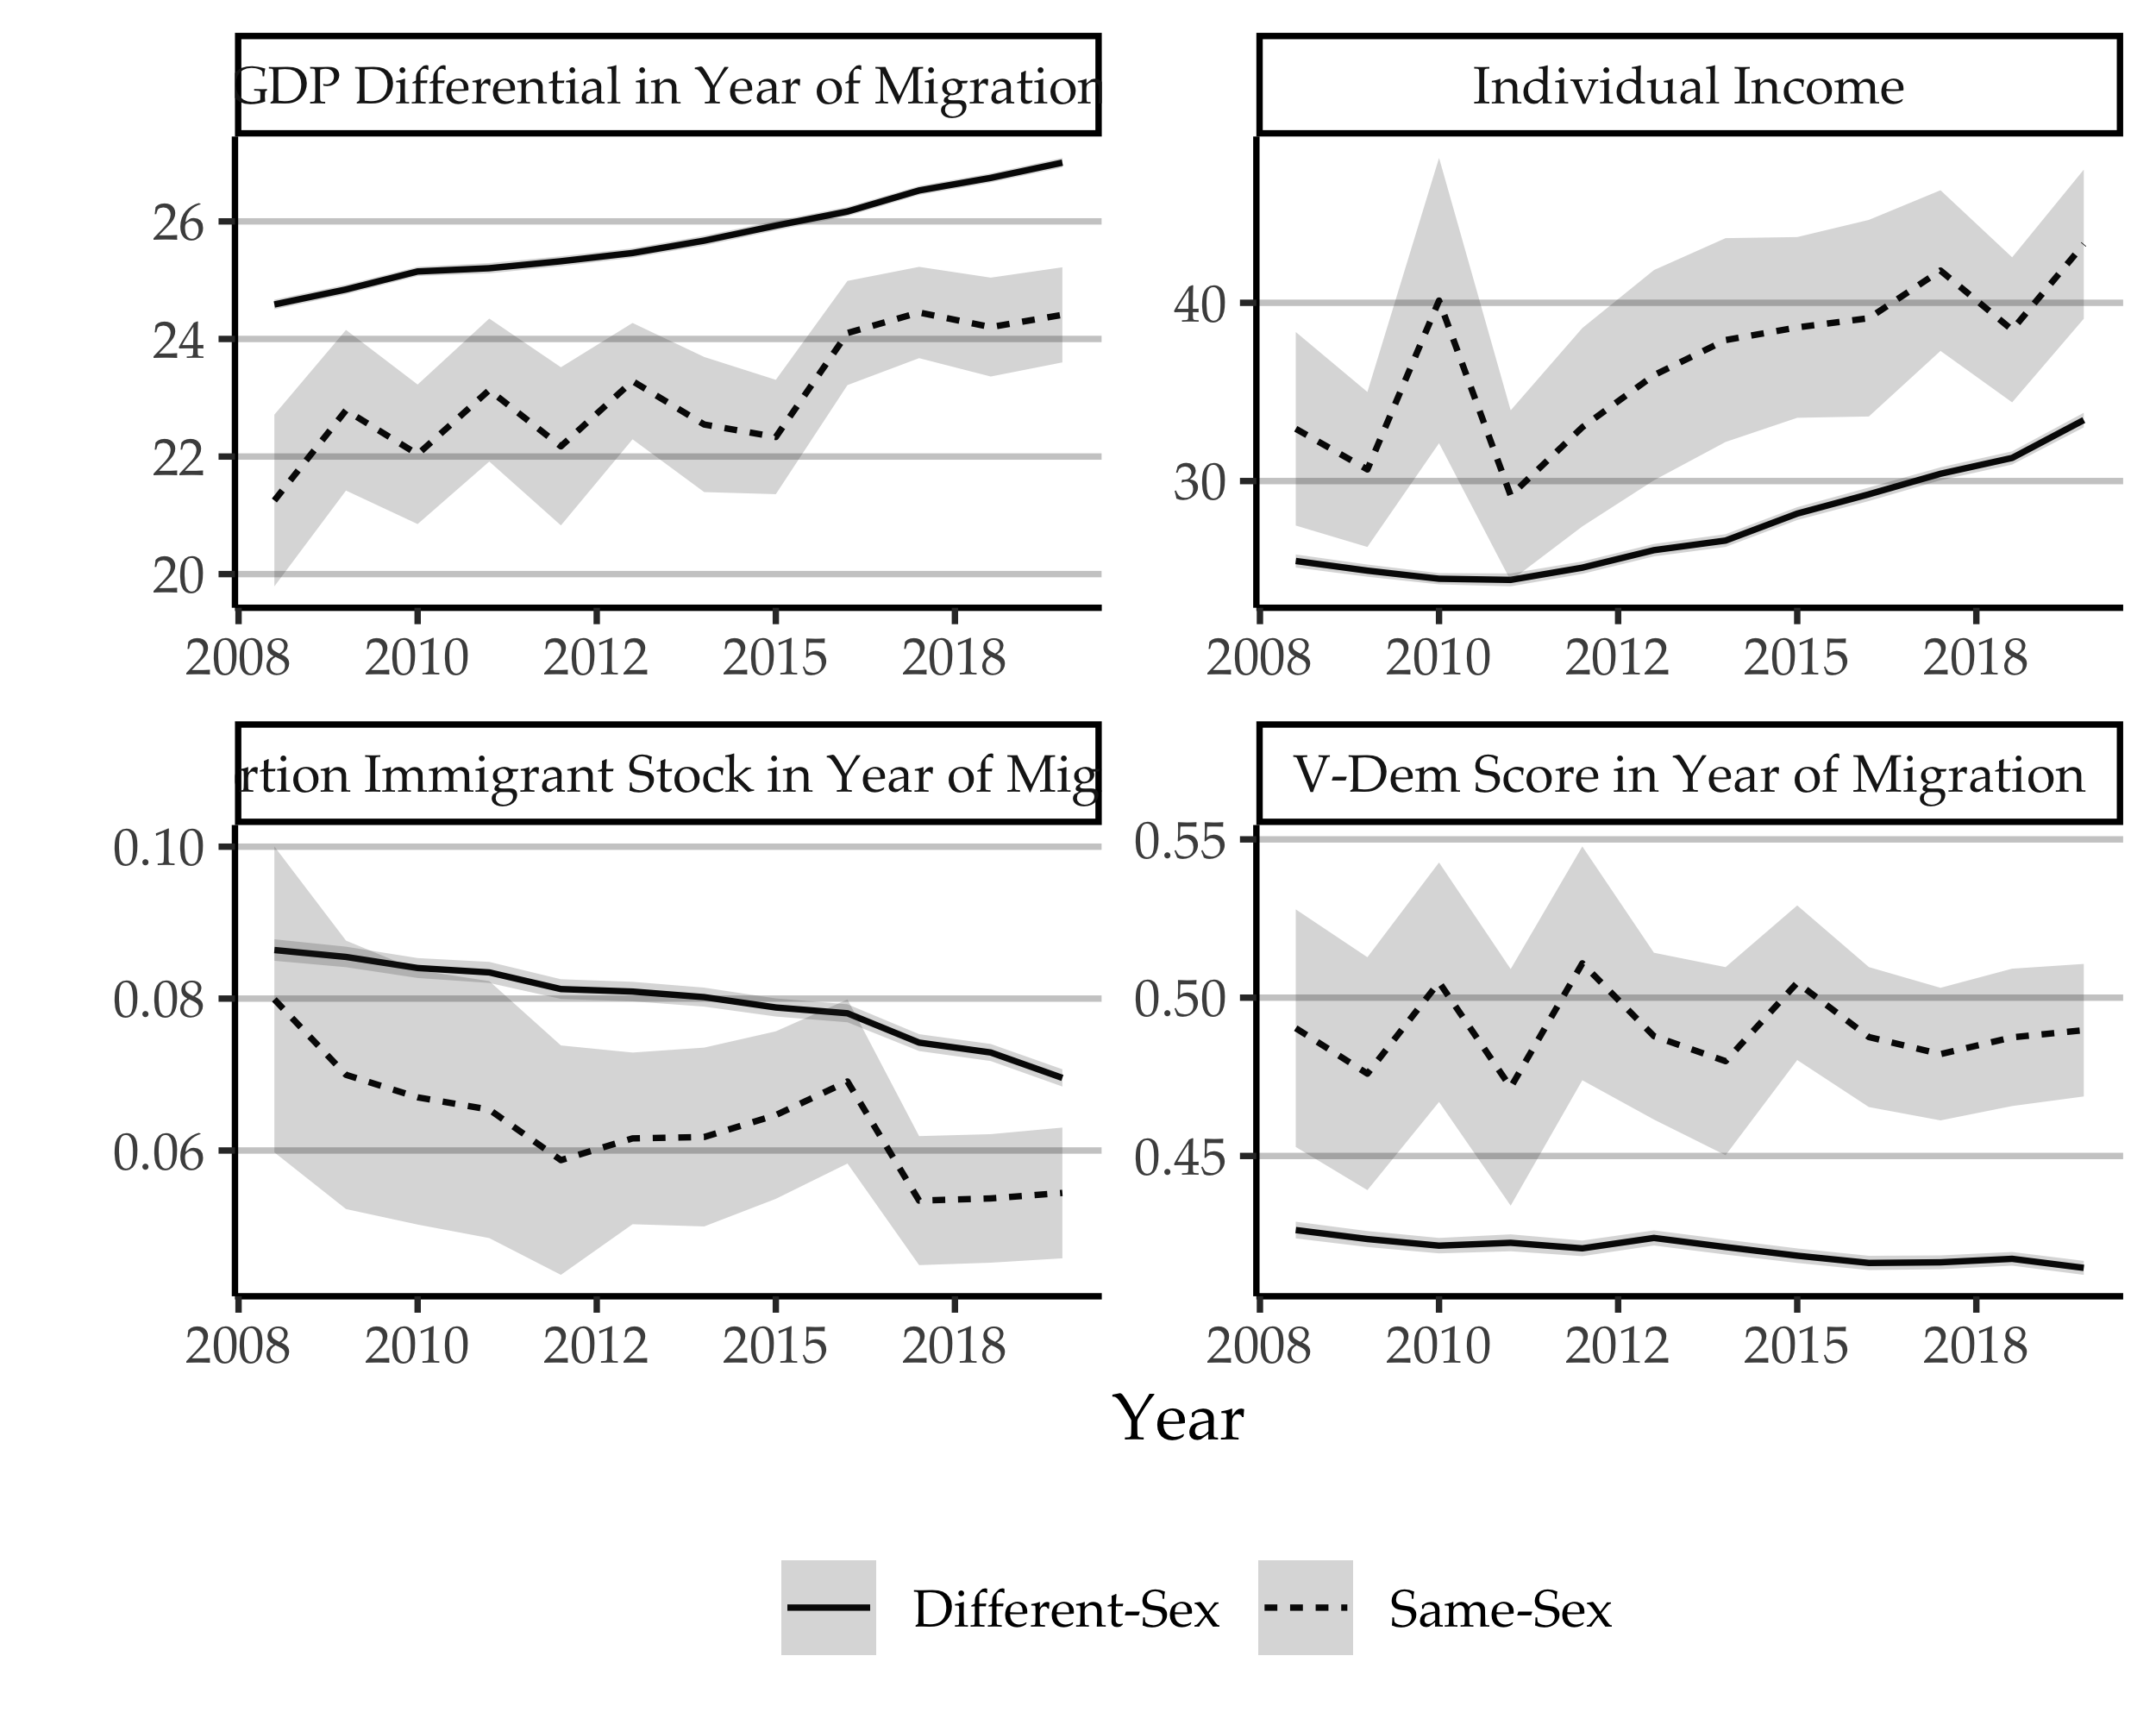
\includegraphics{ssimm_draft_files/figure-latex/desc-1.pdf}
\caption{\label{fig:desc}Descriptive statistics for immigrants in couples 2008-2019, with survey weights and 95\% confidence intervals. All currency in thousands of 1999 dollars.}
\end{figure}

How do same- and different-sex immigrant couples differ in their individual attributes? Do variables typically used in gravity models for migration differ between the groups? Figure \ref{fig:desc} compares immigrants in same- and different-sex couples on four variables. First, macroeconomic theory predicts that difference in wages across countries is one of the most important motivations for migration. The first panel in Figure \ref{fig:desc} shows that the wage differential is indeed positive for both groups of immigrants, but it is significantly more positive for immigrants in different-sex couples. Statistics for the unemployment rate differential (see Supplementary Material) indicate similar trends: LGB immigrants come from countries with lower unemployment rates. These findings indicate that macroeconomic considerations may be less important to the migration of LGB immigrants. The second panel corroborates this finding on the individual level: Not only do immigrants in same-sex couples come from countries with higher per capita GDP, but they individually tend to earn more than immigrants in different-sex couples. Additional analyses (see Supplementary Material) demonstrate that immigrants in same-sex couples also tend to work in professions with higher occupational prestige scores and have somewhat higher education qualifications, indicating that they may come from more privileged social origins than their heterosexual counterparts.

The bottom-left panel of Figure \ref{fig:desc} compares Polity5 democracy level of country of origin at time of migration for immigrants in our study. We see that levels of democracy tend to be higher for immigrants in same-sex couples, indicating that political context may play a more important or different role in their migration. Finally, the fourth panel of Figure \ref{fig:desc} looks at a measure of network effects: at the time of immigration, what is the proportion of total immigrants in the U.S. from the country of origin of members of our sample? Compared to different-sex couples, immigrants in same-sex couples immigrated from countries that were less represented in the U.S. population at the time of migration. This indicates that the network effects that attract migrants from the same country of origin may be less relevant to LGB immigrants.

Although we see significant differences between same- and different-sex couples on a number of important migration variables, none shows the sudden jump in recent years reflected in Figure \ref{fig:total-pop}. Turning to LGBT policy may better explain this surge. Figure \ref{fig:policy-desc} charts the average country-of-origin and U.S.-state LGBT policy score for the immigrants in our sample over time, comparing means for immigrants in same- and different-sex couples. The left panel shows that country-of-origin index at time of migration is generally higher for immigrants in same-sex couples, and since 2013 it has rapidly increased. Immigrants in same-sex couples tend to come from more progressive countries, and this trend tracks closely with the overall population of this group. The right panel indicates less of a difference in U.S. state policies, although states where immigrants in same-sex couples live tend to score somewhat higher.

\begin{figure}
\centering
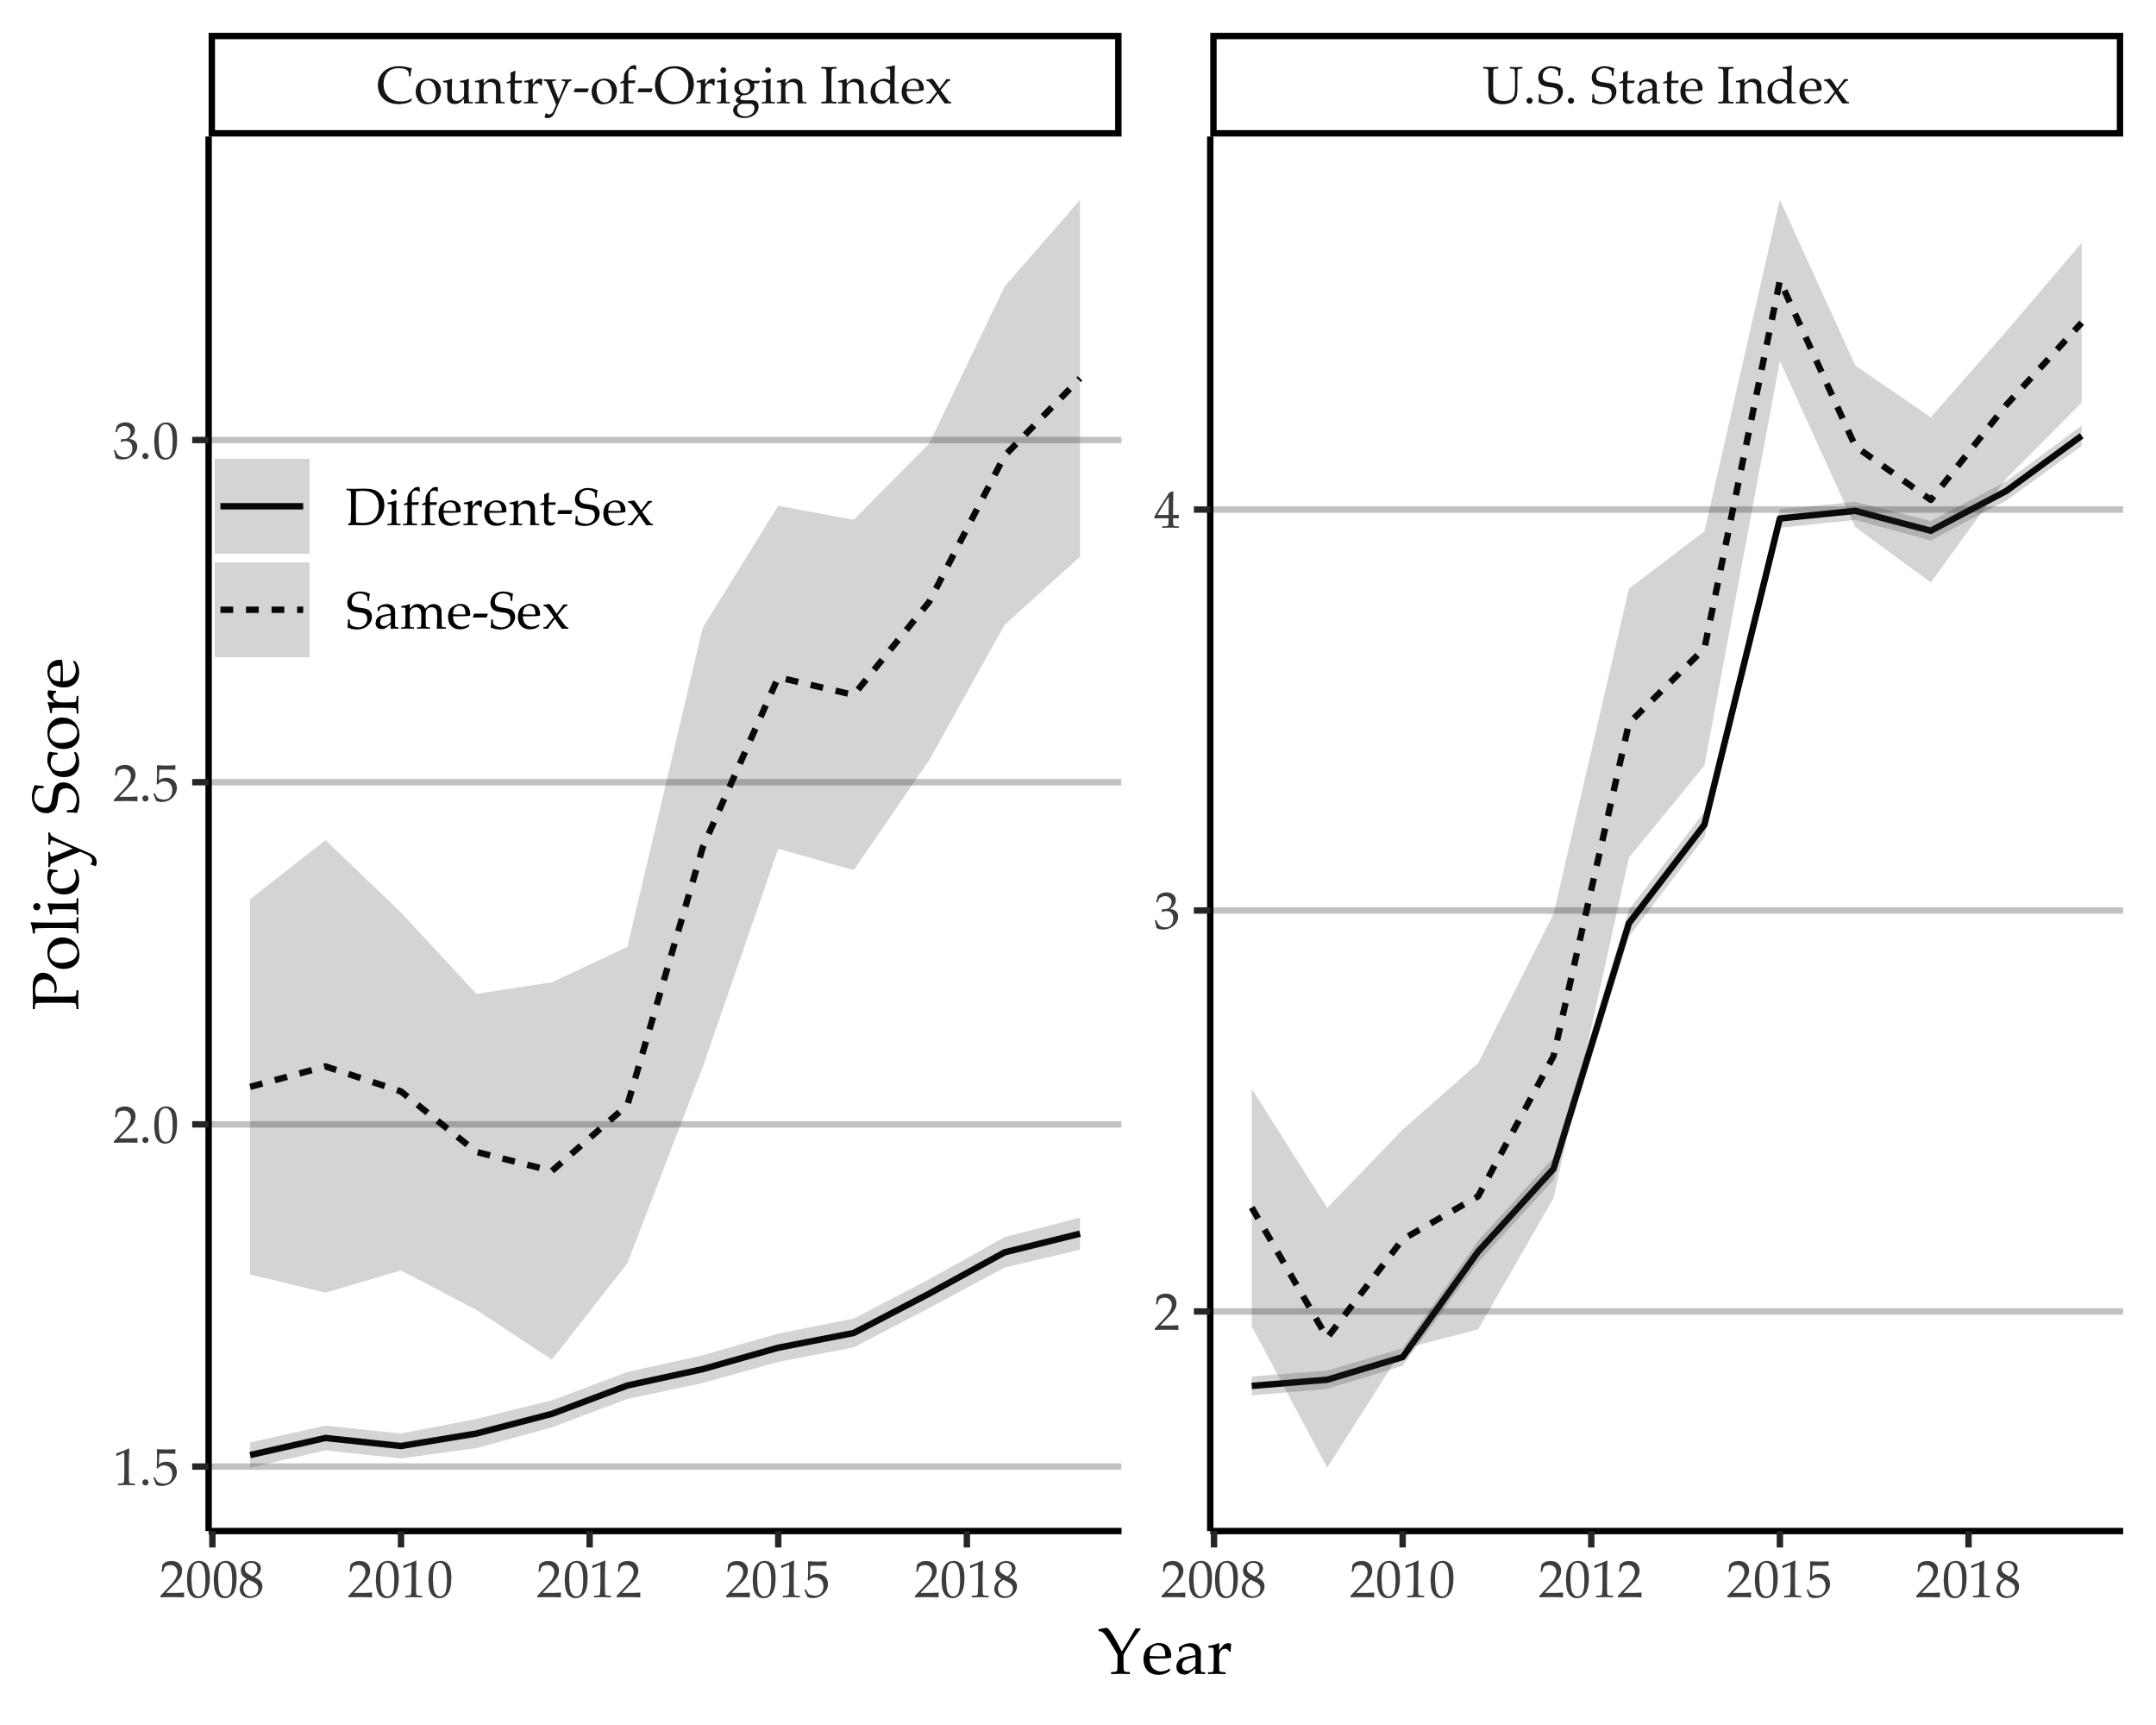
\includegraphics{ssimm_draft_files/figure-latex/policy-desc-1.pdf}
\caption{\label{fig:policy-desc}Mean country-of-origin and U.S. state policy index score for immigrants in same- and different-sex couples, 2008-2019, with 95\% confidence intervals.}
\end{figure}

\begin{table}

\caption{\label{tab:country-tab}Sending countries ranked by proportion immigrant couples with same-sex partners}
\centering
\begin{tabular}[t]{lllr}
\toprule
Rank & Country of origin & Proportion same-sex & Mean policy score\\
\midrule
1 & Belgium & 2.98 \% & 6.30\\
2 & Australia & 2.72 \% & 5.08\\
3 & Netherlands & 2.6 \% & 9.24\\
4 & Malaysia & 2.55 \% & -0.90\\
5 & Bahamas & 2.43 \% & 0.85\\
6 & Mongolia & 2.41 \% & 2.26\\
7 & Zimbabwe & 2.38 \% & -0.96\\
8 & New Zealand & 2.37 \% & 6.99\\
9 & Finland & 2.35 \% & 5.67\\
10 & Singapore & 2.34 \% & 0.10\\
\bottomrule
\multicolumn{4}{l}{\rule{0pt}{1em}\textit{Source:} American Community Survey 2008-2019. Authors' calculations.}\\
\end{tabular}
\end{table}

\begin{table}

\caption{\label{tab:state-tab}States ranked by proportion immigrant couples with same-sex partners}
\centering
\begin{tabular}[t]{lllr}
\toprule
Rank & State & Proportion same-sex & Mean policy score\\
\midrule
1 & Vermont & 2.10 \% & 5.26\\
2 & Maine & 1.51 \% & 4.86\\
3 & Montana & 1.47 \% & 0.94\\
4 & Missouri & 1.11 \% & 1.96\\
5 & Massachusetts & 1.10 \% & 4.80\\
6 & New York & 1.08 \% & 4.90\\
7 & Florida & 0.99 \% & 1.00\\
8 & New Hampshire & 0.95 \% & 4.40\\
9 & Minnesota & 0.92 \% & 4.67\\
10 & New Mexico & 0.92 \% & 4.80\\
\bottomrule
\multicolumn{4}{l}{\rule{0pt}{1em}\textit{Source:} American Community Survey 2008-2019. Authors' calculations.}\\
\end{tabular}
\end{table}

Table \ref{tab:country-tab} ranks the proportion of U.S. immigrants in same-sex couples based on country of origin, averaging over the 11 years of survey data. The top sending countries incorporates interesting diversity. Though there are a number of Western countries with more progressive policies in year of departure for immigrants in our sample, notably, Singapore, Malaysia, and Zimbabwe are also in the top 10. Having countries within the top 10 span multiple regions and cultures gives initial support that responses to ACS questions are not being significantly altered due to these differences. Nor does it appear as though responses to the ACS are just a function of country-of-origin LGBT policies as these also vary significantly across the top 10. Table \ref{tab:state-tab} similarly ranks U.S. state by the proportion of immigrants in same-sex couples, averaging over the period of interest. Although states with progressive policies make the top of the list, Montana, Missouri, and Florida still make the list with less affirming policy environments.

\hypertarget{model-results}{%
\subsection{Model Results}\label{model-results}}

\hypertarget{country-of-origin-effects}{%
\subsubsection{Country-of-Origin Effects}\label{country-of-origin-effects}}

Our first set of models predicts the percent of immigrants in same-sex couples by country of origin and year of immigration (Table \ref{tab:country-props}). Model 1 regresses this proportion on only our variable of interest, LGBT policy score in country of origin. We see that countries with more progressive LGBT policies tend to send more immigrants to the U.S. who end up in same-sex couples. The average country-level proportion of immigrants in same-sex couples is only 0.48 percent, so an increase of 0.037 percent per point increase in LGBT policy score represents a substantive effect.

Models 2 and 3 in Table \ref{tab:country-props} assess the robustness of this finding. Model 2 includes controls from gravity models, including economic differentials, distance, immigrant networks, and democracy. The coefficient for country-of-origin score reduces slightly but remains highly significant. Notably, it is estimated to be more than twice the effect size of the score for democracy; the LGBT policy environment matters much more than the overall progressiveness of government policy. Model 3 adds country-of-origin fixed effects. Although in this model coefficient for origin score is reduced by half compared to Model 1, it remains statistically significant.

\begin{table}[!htbp] \centering 
  \caption{OLS regressions of percent of immigrants in same-sex couples by year of immigration and country of origin. Country-clustered standard errors shown in parentheses. Country controls include population-weighted distance, contiguous border, common official language, common ethnic language, colonial relationship, wage differential, unemployment differential, proportion same-country stock, and democracy.} 
  \label{tab:country-props} 
\begin{tabular}{@{\extracolsep{5pt}}lccccc} 
\\[-1.8ex]\hline 
\hline \\[-1.8ex] 
 & \multicolumn{5}{c}{\textit{Dependent variable:}} \\ 
\cline{2-6} 
\\[-1.8ex] & \multicolumn{5}{c}{Percent in same-sex couples by country-year} \\ 
\\[-1.8ex] & (1) & (2) & (3) & (4) & (5)\\ 
\hline \\[-1.8ex] 
 Country LGBT policy score & 0.037$^{***}$ & 0.036$^{***}$ & 0.021$^{***}$ & $-$0.006 & $-$0.015$^{*}$ \\ 
  & (0.004) & (0.005) & (0.005) & (0.005) & (0.006) \\ 
  & & & & & \\ 
 Polity5 democracy score &  & 0.003 & $-$0.002 & 0.001 & 0.001 \\ 
  &  & (0.002) & (0.002) & (0.002) & (0.002) \\ 
  & & & & & \\ 
 Post-2013 &  &  &  & 0.310$^{***}$ & 0.250$^{***}$ \\ 
  &  &  &  & (0.022) & (0.034) \\ 
  & & & & & \\ 
 Country score × Post-2013 &  &  &  &  & 0.026$^{**}$ \\ 
  &  &  &  &  & (0.010) \\ 
  & & & & & \\ 
\hline \\[-1.8ex] 
Country controls? & no & yes & yes & yes & yes \\ 
Country FEs? & no & no & yes & yes & yes \\ 
Observations & 30,078 & 30,078 & 30,078 & 30,078 & 30,078 \\ 
\hline 
\hline \\[-1.8ex] 
\multicolumn{6}{l}{Note: †p<0.1; *p<0.05; **p<0.01; ***p<0.001} \\ 
\multicolumn{6}{l}{Source: American Community Survey 2008-2019} \\ 
\end{tabular} 
\end{table}

Models 4 and 5 assess how the 2013 Supreme Court decision striking down DOMA figures into these processes. Model 4 is the same as Model 3, but with a dichotomous ``Post-2013'' variable added. The influence of sending-country policy loses its significance in this model: 2013 was a significant turning point for LGB immigrants to the U.S., with the average representation from a given country growing by a quarter of a percent. Model 5 adds an interaction between sending-country LGBT policy score and the post-2013 dichotomous variable. This variable is significant and positive, while the other variables of interest lose significance. Sending-country policy and the post-2013 era both matter, but solely in tandem: Only LGB immigrants from progressive countries see a boost in representation after the DOMA decision.\footnote{The Supplementary Material also includes a model with only married couples and one with only couples that include one immigrant and one U.S.-born citizen. Results are nearly identical to models fit to the full sample.}

\begin{table}[!htbp] \centering 
  \caption{Percent same-sex in by country of origin, U.S. state, and survey year. Country-clustered standard errors are shown in parentheses. State controls include unemployment rate and per-capita income. Country controls include population-weighted distance, contiguous border, common official language, common ethnic language, colonial relationship, wage differential, unemployment differential, proportion same-country stock, and democracy.} 
  \label{tab:state-props} 
\begin{tabular}{@{\extracolsep{5pt}}lcccccc} 
\\[-1.8ex]\hline 
\hline \\[-1.8ex] 
 & \multicolumn{6}{c}{\textit{Dependent variable:}} \\ 
\cline{2-7} 
\\[-1.8ex] & \multicolumn{6}{c}{Percent in same-sex couples by state-country-year} \\ 
\\[-1.8ex] & (1) & (2) & (3) & (4) & (5) & (6)\\ 
\hline \\[-1.8ex] 
 State LGBT policy score & 0.063$^{***}$ & 0.058$^{***}$ & 0.026 & 0.015 & $-$0.002 & 0.002 \\ 
  & (0.016) & (0.016) & (0.035) & (0.035) & (0.035) & (0.036) \\ 
  & & & & & & \\ 
 Country LGBT policy score &  & 0.078$^{***}$ & 0.071$^{***}$ & 0.120$^{**}$ & 0.090$^{*}$ & $-$0.007 \\ 
  &  & (0.009) & (0.009) & (0.038) & (0.039) & (0.047) \\ 
  & & & & & & \\ 
 Post-2013 &  &  &  &  & 0.240$^{***}$ & 0.110 \\ 
  &  &  &  &  & (0.068) & (0.077) \\ 
  & & & & & & \\ 
 Country score × Post-2013 &  &  &  &  &  & 0.075$^{***}$ \\ 
  &  &  &  &  &  & (0.021) \\ 
  & & & & & & \\ 
\hline \\[-1.8ex] 
State controls and FEs? & no & no & yes & yes & yes & yes \\ 
Country controls and FEs? & no & no & no & yes & yes & yes \\ 
Observations & 35,636 & 35,636 & 35,636 & 35,636 & 35,636 & 35,636 \\ 
\hline 
\hline \\[-1.8ex] 
\multicolumn{7}{l}{Note: †p<0.1; *p<0.05; **p<0.01; ***p<0.001} \\ 
\multicolumn{7}{l}{Source: American Community Survey 2008-2019} \\ 
\end{tabular} 
\end{table}

\hypertarget{state-effects}{%
\subsubsection{State Effects}\label{state-effects}}

We next turn to the effects of U.S. state LGBT policy. Table \ref{tab:state-props} presents models of U.S. state-level proportion of immigrants in same-sex couples, from a given country of origin in a given survey year. Model 1 contains only one predictor: U.S. state policy score in the survey year. We see that, on average, states with more friendly LGBT policies have somewhat higher proportions of immigrants in same-sex couples. Model 2 adds a predictor for country-of-origin policy score at the mean year of immigration. Although the coefficient for country of origin score is more precisely estimated, the two variables have effects of roughly equal size. A one-standard deviation (2.2-point) increase origin score is associated with a 0.17 percentage-point increase of immigrants in same-sex couples, whereas the corresponding state policy standard deviation increase of 2.4 points is 0.14 percentage points.

According to the descriptive analysis above, immigrants in same-sex couples tend to have higher incomes and hold more prestigious occupations than immigrants in different-sex couples. This implies that immigrants in same-sex couples may be attracted to progressive states for their economic rather than political benefits, so Model 3 adds state-level controls and fixed effects. Indeed, in this model, the coefficient for state policy is reduced and rendered insignificant. Model 4 adds country-of-origin controls and fixed effects. The state policy effect remains imprecisely estimated, but country-of-origin policy has increased in strength. More progressive sending countries are represented by greater proportions of same-sex couples, while U.S. state policy appears to have little influence on their settlement patterns, at least in the aggregate.

Model 5 includes a dichotomous variable for the post-2013 DOMA decision era, and Model 6 interacts this with sending-country score. Unlike for the country-level models in Table \ref{tab:country-props}, both the time variable and its interaction remain significant in the final model. After 2013, the proportion of immigrants in same-sex couples increased within states, but this was especially true for immigrants from more progressive countries.

\hypertarget{individual-analysis}{%
\subsubsection{Individual Analysis}\label{individual-analysis}}

Our final set of models focuses on the individual. Conditional on migrating to the U.S., do immigrants in same-sex couples choose to live in more progressive states than their heterosexual counterparts? Table \ref{tab:ord} presents ordered logit models predicting whether an individual partnered immigrant lives in a U.S. state with repressive, neutral, or progressive LGBT policies, pooling data across survey years. Model 1 includes only one regressor: an indicator for whether the immigrant is in a same-sex couple. The positive coefficient indicates that immigrants in same-sex couples indeed tend to live in states with more LGBT-friendly policies. The predicted probability for an immigrant in a different-sex couple to live in a state with progressive LGBT policies is 0.55, whereas the corresponding probability for those in same-sex couples is 0.6. At the repressive end of the policy spectrum, the predicted probabilities are 0.24 and 0.2 for different- and same-sex couples, respectively.

How does country-of-origin context mediate this results? Model 2 adds sending-country LGBT policy score at the time of immigration to the regression, interacting it with the same-sex indicator. The coefficient for the same-sex indicator remains positive and significant, but we see opposite effects of the origin-score coefficient for immigrants in different- and same-sex couples. For different-sex couples, hailing from a more progressive country is associated with living in a more repressive U.S. state. For same-sex couples, the result is in the opposite direction: those from progressive countries tend to live in more progressive U.S. states.

Model 3 controls for possible individual confounders, interacting them with the same-sex indicator. If immigrants in same-sex couples also tend to have more education, higher income, different family structures, or less years of age, they may be choosing more progressive states due to other policies or economic conditions. As shown in Table \ref{tab:ord}, our variables of interest remain strong and in the same directions in this final model.

\begin{table}[!htbp] \centering 
  \caption{Individual ordered logit analysis of three-category state policy score. Country-clustered standard errors are shown in parentheses. Individual controls include sex, age, education, number of children, log(income), indicator for no income, and year of immigration, which are all interacted with the indicator for same-sex couple.} 
  \label{tab:ord} 
\begin{tabular}{@{\extracolsep{5pt}}lccc} 
\\[-1.8ex]\hline 
\hline \\[-1.8ex] 
 & \multicolumn{3}{c}{\textit{Dependent variable:}} \\ 
\cline{2-4} 
\\[-1.8ex] & \multicolumn{3}{c}{Binned state LGBT policy score} \\ 
\\[-1.8ex] & (1) & (2) & (3)\\ 
\hline \\[-1.8ex] 
 Same-sex & 0.190$^{***}$ & 0.110$^{**}$ & 21.000$^{***}$ \\ 
  & (0.025) & (0.035) & (0.0004) \\ 
  & & & \\ 
 Country LGBT policy score &  & $-$0.044$^{***}$ & $-$0.030$^{***}$ \\ 
  &  & (0.003) & (0.003) \\ 
  & & & \\ 
 Same-sex × country score &  & 0.041$^{***}$ & 0.051$^{***}$ \\ 
  &  & (0.009) & (0.009) \\ 
  & & & \\ 
\hline \\[-1.8ex] 
Survey year FEs? & yes & yes & yes \\ 
Individual controls? & no & no & yes \\ 
Observations & 107,500 & 107,500 & 107,500 \\ 
\hline 
\hline \\[-1.8ex] 
\multicolumn{4}{l}{Note: †p<0.1; *p<0.05; **p<0.01; ***p<0.001} \\ 
\multicolumn{4}{l}{Source: American Community Survey 2008-2019} \\ 
\end{tabular} 
\end{table}

\begin{figure}
\centering
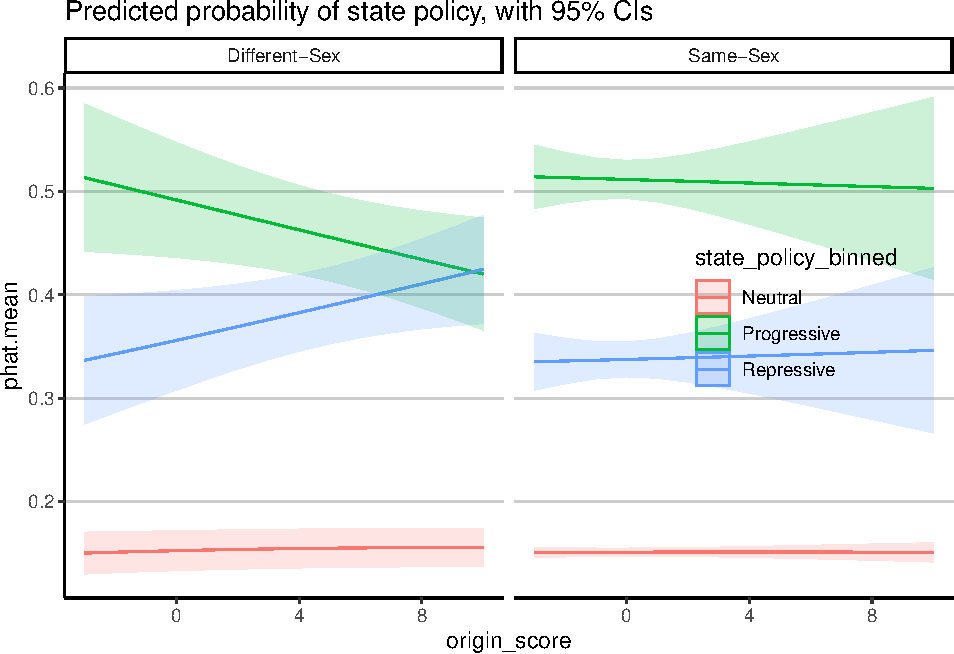
\includegraphics{ssimm_draft_files/figure-latex/sim-1.pdf}
\caption{\label{fig:sim}Predicted probabilities of U.S. state LGBT policy progressiveness for individual immigrants in different- and same-sex couples, based on policy score of sending country, with 95\% confidence intervals.}
\end{figure}

To help interpret these results, Figure \ref{fig:sim} contains predicted probabilities of residing in progressive, neutral, or repressive U.S. states. For each of 250 simulations, the coefficients are drawn from this covariance matrix as estimated in Model 3 in Table \ref{tab:ord}. These are used to predict the probability of being in each type of state for each member in the complete dataset, with their couple type set to same- or different-sex and their origin score varied from the minimum to maximum. The predicted probabilities are are averaged across the entire dataset for each of these manipulated values. After 250 simulations, the distribution of predicted values is used to find means and 95-percent confidence intervals. The only difference between the two panels is the value for the same-sex indicator in the simulations.

The figure shows opposite trends for same- and different-sex couples. Overall, immigrants tend to live in more progressive states, but the moderating effect of origin score is quite different for the two groups. The panel for same-sex couples shows that these immigrants tend to live in U.S. states with similar LGBT policy contexts to those of their countries of origin. Immigrants in same-sex couples from repressive countries are less likely to live in progressive U.S. states, but as the origin-country score increases, so does the probability of living in a progressive state. For immigrants in different-sex couples, on the other hand, increasingly progressive country-of-origin policies are associated with a \emph{lower} probability of residing in a progressive U.S. state, accompanied by a \emph{higher} probability of living in a repressive U.S. state. At the high end of the origin-score policy range, the difference in predicted probabilities is significant: Typical immigrants in same-sex couples are 15 percentage points more likely to live in progressive states and 10 percentage points less likely to live in repressive states than similar immigrants in different-sex couples. Though the pattern for same-sex couples is understandable and expected, the lower probabilities for different-sex couples raises important questions. Regardless, these results demonstrate that sexuality, and the governance of it, influences migration patters for those in both same-sex and different-sex relationships.

\hypertarget{discussion}{%
\section{Discussion}\label{discussion}}

In 2013, there were 61 thousand same-sex couples that included immigrants in the U.S. By 2019, this number had nearly doubled to 107 thousand. Despite this expansive growth of same-sex immigrant couples in the U.S. far outpacing overall migration rates, there is little demographic research understanding the characteristics of these couples or the factors influencing their migratory patterns. The research on queer migrants that does exist is largely qualitative and focused on asylum claims. Consequently, we know little about who these migrants are, why they are choosing to leave their home countries, or where they are choosing to locate once in the U.S. Answering these questions is important, not just because this represents an increasing number of border crossers, but because this process has the potential to reshape our conceptualization of who immigrants are, their motivations for moving, and how policy apparently unrelated to migration can shape the aspirations and capacities of would-be migrants (\protect\hyperlink{ref-dehaas_2021}{de Haas, 2021}).

The rising number of same-sex immigrant couples has coincided with a dramatic change in policy environments governing LGBT communities, both within the U.S. and abroad. Thanks to the 2013 DOMA Supreme Court case, same-sex couples now have a broader legal pathway into the U.S. (\protect\hyperlink{ref-edwards_2013}{Edwards, 2013}). Therefore, although there are numerous perspectives to take in understanding the migratory patterns of these couples, this project investigates how changing LGBT policies at both country of origin and residing U.S. state pattern these migratory pathways. Engaging in such a question adds to emerging scholarship trying to understand how dramatic policy changes are influencing the health, well-being, and lifestyles of LGBT people while also recognizing that these policies differentially impact people within this broad umbrella based on different social positions (\protect\hyperlink{ref-boertien_2019}{Boertien \& Vignoli, 2019}; \protect\hyperlink{ref-carpenter_2020}{Carpenter, 2020}; \protect\hyperlink{ref-kail_2015}{Kail et al., 2015}; \protect\hyperlink{ref-levy_2017}{Levy \& Levy, 2017}). Moreover, this project helps address an important gap within migration studies, a field that too often discounts the role of the state and the salience of sexuality in conditioning migratory patterns (\protect\hyperlink{ref-carrillo_2018}{Carrillo, 2018}; \protect\hyperlink{ref-fitzgerald_2014}{Fitzgerald et al., 2014}).

To answer our questions, we take advantage of an underutilized data source: self-reports of same-sex immigrant couples in the American Community Survey from 2008 to 2019. Despite this resource being one of the few national surveys to identify same-sex immigrant couples, these data are virtually untapped for this purpose. In light of possible reporting issues with these data (\protect\hyperlink{ref-gates_2013}{Gates, 2013a}; \protect\hyperlink{ref-goodnature_2021}{Goodnature \& Neto, 2021}), in the Supplemental Material we probe the sensitivity of our findings only to find remarkable robustness to high levels of misreporting. As such, these data allow for us to make one of the first large-\(N\) investigations of same-sex immigrant couples within the U.S. and to make an important addition to this area of scholarship, even descriptively.

Using these data, we make a number of findings worth detailing. First, existing scholarship on same-sex immigrant couples, and queer migration more broadly, largely focuses on the asylum and refugee processes (\protect\hyperlink{ref-luibheid_2008}{Luibhéid, 2008}; \protect\hyperlink{ref-vogler_2016}{Vogler, 2016}). This is because this was one of the only mechanisms for getting into the U.S. (\protect\hyperlink{ref-humanrightswatch_2006}{Human Rights Watch, 2006}). Furthermore, even research on non-refugee LGB immigrants tends to select cases from relatively repressive contexts (\protect\hyperlink{ref-cantu_2009}{Cantú, 2009}; \protect\hyperlink{ref-carrillo_2018}{Carrillo, 2018}). Consequently, this over-representation distorts our understanding of who same-sex immigrant couples are, the types of environments they are leaving, and their motivations to seek entry into the U.S. Indeed, when comparing the demographics of same-sex immigrant couples to different-sex immigrant couples, we find same-sex couples generally have higher incomes and occupational prestige and are somewhat more educated. Understanding this profile alone is an important insight as it reveals that these communities are of privileged social standing. This is a corrective to the queer migration literature that has yet to highlight this profile.

Understanding who these migrants are, how do LGBT policies in their countries-of-origin influence their desires to come to the U.S.? Despite existing scholarship portraying a story of LGB couples fleeing repression, as necessary for refugee claims, LGB couples are leaving countries with more progressive policy environments. As results in Table \ref{tab:country-props} and trendlines in Figure \ref{fig:policy-desc} reveal, couples are coming from more open environments. This is true even after accounting for traditional gravity model explanations that primarily focus on economic costs and benefits and established sociological determinants like networks and cultural proximity. Though more research is needed, these results, in conjunction with the fact that these same-sex couples achieve higher incomes and greater occupational prestige, describe a situation in which perhaps it is a supportive policy environment, such as employment protections, access to the material benefits of marriage, and so forth, that enable same-sex couples to achieve greater social standing and the resources necessary to migrate. Or, instead of the immediate benefits of the policy itself, these supportive environments may simply encourage LGB people to feel comfortable openly identifying as being in a relationship when responding to surveys. Regardless, it appears that same-sex couples are more apt to follow the lifestyle migration pathways and motivations when coming to the U.S. as opposed to explicitly trying to leave more repressive contexts in hopes of living more open lives.

One unexpected finding is that different-sex couples from more LGBT-friendly countries are likelier to reside in states with increasingly less LGBT-friendly policies. These patterns in Figure \ref{fig:sim} are peculiar because we suspected that state LGBT policies to have no association with how different-sex couples are making decisions as to where to reside. This is not the case. One immediate question this raises is if this is a case of ``straight flight.'' White flight is a well-research process in which white people leave diversifying communities. After straight couples experience liberalized conditions for gay couples, do they intentionally seek to leave such conditions by moving to states that are less supportive? Alternatively, it may be that the economic and social forces pulling different-sex immigrants to these particular states may spuriously be associated with less progressive LGBT policies. More research is needed to understand this interesting pattern.

Recent research has argued that sexuality is a salient factor determining immigration decisions. We show that differences between immigrants in same-sex couples and those in different-sex couples cannot be explained solely using classic theories of migration; policy context and sexuality interact in complicated ways to shape migratory flows. Though our primary focus is on same-sex couples, this study contributes toward the broader literature offering a correction to standard models of migration. Lifestyle migration is often used to describe affluent people moving in search of a better way of life (\protect\hyperlink{ref-benson_2009}{Benson \& O'Reilly, 2009}). But what the present scholarship contributes is that sexuality shapes how that ``better way of life'' is conceptualized and motivated, contributing toward our understanding these dynamics (\protect\hyperlink{ref-dixon_2020}{Dixon, 2020}). The present findings raise additional questions as to how sexuality motivates migration patterns and are (in)directly influencing seemingly economic or networked dynamics, even for heterosexual couples. Finally, to borrow the line from Theda Skocpol, we are ``bringing the state back in'' (\protect\hyperlink{ref-skocpol_1985}{Skocpol et al., 1985}). Typically, state policies are less integrated within models of migration. When they are, the policies under examination are usually those specific to migration. But what this study demonstrates is that, for same-sex couples, once the legal opening to migration occurred after the DOMA ruling, it was policy specific to LGBT issues, rather than just migration, that influenced their ``push'' to the U.S. This opens up questions as to how state policies relative to a particular group, but not explicitly in the domain of immigration, create structural conditions for which some communities choose to leave their home country. This points to the importance of further studying identity, and the state's governance of it, in migratory processes.

\hypertarget{references}{%
\section{References}\label{references}}

\setlength{\parindent}{-0.2in}
\setlength{\leftskip}{0.2in}
\setlength{\parskip}{8pt}

\noindent

\hypertarget{refs}{}
\begin{CSLReferences}{1}{0}
\leavevmode\hypertarget{ref-adur_2018}{}%
Adur, S. M. (2018). In pursuit of love: {`{Safe} passages,'} migration and queer {South Asians} in the {US}. \emph{Current Sociology}, \emph{66}(2), 320--334.

\leavevmode\hypertarget{ref-ahmad_2013}{}%
Ahmad, P. A. N. (2013). Sexuality and {Migration}: {Thinking} beyond the {Economic}. In \emph{Masculinity, {Sexuality} and {Illegal Migration}: {Human Smuggling} from {Pakistan} to {Europe}} (pp. 67--93). {Ashgate Publishing, Ltd.}

\leavevmode\hypertarget{ref-anderson_2011}{}%
Anderson, J. E. (2011). The {Gravity Model}. \emph{Annual Review of Economics}, \emph{3}(1), 133--160. \url{https://doi.org/10.1146/annurev-economics-111809-125114}

\leavevmode\hypertarget{ref-ayoub_2016}{}%
Ayoub, P. (2016). \emph{When {States Come Out}}. {Cambridge University Press}.

\leavevmode\hypertarget{ref-ayoub_2017}{}%
Ayoub, P., \& Garretson, J. (2017). Getting the message out: {Media} context and global changes in attitudes toward homosexuality. \emph{Comparative Political Studies}, \emph{50}(8), 1055--1085.

\leavevmode\hypertarget{ref-baumle_2009}{}%
Baumle, A. K., Compton, D., \& Poston, D. L. (2009). \emph{Same-{Sex Partners}: {The Social Demography} of {Sexual Orientation}}. {SUNY Press}.

\leavevmode\hypertarget{ref-bea_2020}{}%
BEA. (2020). \emph{Regional {Data}: {GDP} and {Personal Income}}. {Bureau of Economic Analysis, U.S. Department of Commerce}.

\leavevmode\hypertarget{ref-beaudin_2017}{}%
Beaudin, L. (2017). Marriage equality and interstate migration. \emph{Applied Economics}, \emph{49}(30), 2956--2973. \url{https://doi.org/10.1080/00036846.2016.1251565}

\leavevmode\hypertarget{ref-beine_2016}{}%
Beine, M., Bertoli, S., \& Moraga, J. F.-H. (2016). A {Practitioners}' {Guide} to {Gravity Models} of {International Migration}. \emph{The World Economy}, \emph{39}(4), 496--512. \url{https://doi.org/10.1111/twec.12265}

\leavevmode\hypertarget{ref-benson_2016}{}%
Benson, M., \& O'Reilly, K. (2016). From lifestyle migration to lifestyle in migration: {Categories}, concepts and ways of thinking. \emph{Migration Studies}, \emph{4}(1), 20--37. \url{https://doi.org/10.1093/migration/mnv015}

\leavevmode\hypertarget{ref-benson_2009}{}%
Benson, M., \& O'Reilly, K. (2009). Migration and the {Search} for a {Better Way} of {Life}: {A Critical Exploration} of {Lifestyle Migration}. \emph{The Sociological Review}, \emph{57}(4), 608--625. \url{https://doi.org/10.1111/j.1467-954X.2009.01864.x}

\leavevmode\hypertarget{ref-benson_2012}{}%
Benson, M., \& O'Reilly, K. (2012). \emph{Lifestyle {Migration}: {Expectations}, {Aspirations} and {Experiences}} (Har/Ele edition). {Ashgate}.

\leavevmode\hypertarget{ref-bls_2020}{}%
BLS. (2020). \emph{Monthly state unemployment rates}. {U.S. Bureau of Labor Statistics}.

\leavevmode\hypertarget{ref-boertien_2019}{}%
Boertien, D., \& Vignoli, D. (2019). Legalizing same-sex marriage matters for the subjective well-being of individuals in same-sex unions. \emph{Demography}, \emph{56}(6), 2109--2121.

\leavevmode\hypertarget{ref-canaday_2009}{}%
Canaday, M. (2009). \emph{The straight state: Sexuality and citizenship in twentieth-century {America}}. {Princeton University Press}.

\leavevmode\hypertarget{ref-cantu_2009}{}%
Cantú, L. (2009). \emph{The {Sexuality} of {Migration}: {Border Crossings} and {Mexican Immigrant Men}} (N. A. Naples \& S. Vidal-Ortiz, Eds.). {NYU Press}.

\leavevmode\hypertarget{ref-carpenter_2020}{}%
Carpenter, C. S. (2020). The {Direct Effects} of {Legal Same}-{Sex Marriage} in the {United States}: {Evidence From Massachusetts}. \emph{Demography}, \emph{57}(5), 1787--1808.

\leavevmode\hypertarget{ref-carrillo_2018}{}%
Carrillo, H. (2018). \emph{Pathways of {Desire}: {The Sexual Migration} of {Mexican Gay Men}}. {University of Chicago Press}.

\leavevmode\hypertarget{ref-christafore_2019}{}%
Christafore, D., \& Leguizamon, S. (2019). Taste-{Based Discrimination}, {Tolerance} and the {Wage Gap}: {When Does Economic Freedom Help Gay Men}? \emph{Kyklos}, \emph{72}(3), 426--445. \url{https://doi.org/10.1111/kykl.12206}

\leavevmode\hypertarget{ref-corey-boulet_2019}{}%
Corey-Boulet, R. (2019). \emph{Love {Falls On Us}: {A Story} of {American Ideas} and {African LGBT Lives}}. {Zed Books Ltd.}

\leavevmode\hypertarget{ref-dehaas_2021}{}%
de Haas, H. (2021). A theory of migration: The aspirations-capabilities framework. \emph{Comparative Migration Studies}, \emph{9}(1), 8. \url{https://doi.org/10.1186/s40878-020-00210-4}

\leavevmode\hypertarget{ref-dixon_2020}{}%
Dixon, L. (2020). Gender, sexuality and lifestyle migration: {Exploring} the impact of cosmopolitan place-marketing discourses on the post-migratory experiences of {British} women in {Spain}. \emph{Current Sociology}, \emph{68}(3), 281--298. \url{https://doi.org/10.1177/0011392119850231}

\leavevmode\hypertarget{ref-edwards_2013}{}%
Edwards, B. P. (2013). Welcoming a {Post}-{DOMA World}: {Same}-{Sex Spousal Petitions} and {Other Post}-{Windsor Immigration Implications}. \emph{Family Law Quarterly}, \emph{47}(2), 173--189.

\leavevmode\hypertarget{ref-epstein_2014}{}%
Epstein, S., \& Carrillo, H. (2014). Immigrant sexual citizenship: Intersectional templates among {Mexican} gay immigrants to the {USA}. \emph{Citizenship Studies}, \emph{18}(3-4), 259--276. \url{https://doi.org/10.1080/13621025.2014.905266}

\leavevmode\hypertarget{ref-feenstra_2015}{}%
Feenstra, R. C., Inklaar, R., \& Timmer, M. P. (2015). The {Next Generation} of the {Penn World Table}. \emph{American Economic Review}, \emph{105}(10), 3150--3182. \url{https://doi.org/10.1257/aer.20130954}

\leavevmode\hypertarget{ref-feliciano_2020}{}%
Feliciano, C. (2020). Immigrant {Selectivity Effects} on {Health}, {Labor Market}, and {Educational Outcomes}. \emph{Annual Review of Sociology}, \emph{46}(1), 315--334. \url{https://doi.org/10.1146/annurev-soc-121919-054639}

\leavevmode\hypertarget{ref-fisher_2018}{}%
Fisher, R., Gee, G., \& Looney, A. (2018). Same-{Sex Married Tax Filers After Windsor} and {Obergefell}. \emph{Demography}, \emph{55}(4), 1423--1446. \url{https://doi.org/10.1007/s13524-018-0684-5}

\leavevmode\hypertarget{ref-fitzgerald_2014}{}%
Fitzgerald, J., Leblang, D., \& Teets, J. C. (2014). Defying the {Law} of {Gravity}: {The Political Economy} of {International Migration}. \emph{World Politics}, \emph{66}(3), 406--445. \url{https://doi.org/10.1017/S0043887114000112}

\leavevmode\hypertarget{ref-gates_2013}{}%
Gates, G. J. (2013a). \emph{{LGBT Adult Immigrants} in the {United States}}. {The Williams Institute}.

\leavevmode\hypertarget{ref-gates_2013a}{}%
Gates, G. J. (2013b). Geography of the {LGBT} population. In \emph{International handbook on the demography of sexuality} (pp. 229--242). {Springer}.

\leavevmode\hypertarget{ref-gates_2009}{}%
Gates, G. J., \& Steinberger, M. D. (2009). Same-sex unmarried partner couples in the {American Community Survey}: {The} role of misreporting, miscoding and misallocation. \emph{Annual Meetings of the Population Association of America, Detroit, {MI}}.

\leavevmode\hypertarget{ref-giametta_2020}{}%
Giametta, C. (2020). New asylum protection categories and elusive filtering devices: The case of {`{Queer} asylum'} in {France} and the {UK}. \emph{Journal of Ethnic and Migration Studies}, \emph{46}(1), 142--157.

\leavevmode\hypertarget{ref-goldberg_2021}{}%
Goldberg, S. K., \& Conron, K. J. (2021). \emph{{LGBT Adult Immigrants} in the {United States}}. {The Williams Institute}.

\leavevmode\hypertarget{ref-gonzalez-lopez_2005}{}%
González-López, G. (2005). \emph{Erotic {Journeys}}. {University of California Press}.

\leavevmode\hypertarget{ref-goodnature_2021}{}%
Goodnature, M., \& Neto, A. B. F. (2021). Same-{Sex Unmarried Partners} in the {Census}. \emph{Journal of Regional Analysis \& Policy}, \emph{51}(1), 43--66.

\leavevmode\hypertarget{ref-gorman-murray_2009}{}%
Gorman-Murray, A. (2009). Intimate mobilities: Emotional embodiment and queer migration. \emph{Social \& Cultural Geography}, \emph{10}(4), 441--460. \url{https://doi.org/10.1080/14649360902853262}

\leavevmode\hypertarget{ref-hatton_2005a}{}%
Hatton, T. J., \& Williamson, J. G. (2005). \emph{Global {Migration} and the {World Economy}: {Two Centuries} of {Policy} and {Performance}}. {The MIT Press}. \url{https://doi.org/10.7551/mitpress/3303.001.0001}

\leavevmode\hypertarget{ref-hondagneu-sotelo_2012}{}%
Hondagneu-Sotelo, P. (2012). New directions in gender and immigration research. In \emph{Routledge {International Handbook} of {Migration Studies}}. {Routledge}. \url{https://doi.org/10.4324/9780203863299.ch15}

\leavevmode\hypertarget{ref-humanrightswatch_2006}{}%
Human Rights Watch. (2006). \emph{Family, {Unvalued}: {Discrimination}, {Denial}, and the {Fate} of {Binational Same}-{Sex Couples} under {U}.{S}. {Law}}.

\leavevmode\hypertarget{ref-kail_2015}{}%
Kail, B. L., Acosta, K. L., \& Wright, E. (2015). State-level marriage equality and the health of same-sex couples. \emph{American Journal of Public Health}, \emph{105}(6), 1101--1105.

\leavevmode\hypertarget{ref-karemera_2000}{}%
Karemera, D., Oguledo, V. I., \& Davis, B. (2000). A gravity model analysis of international migration to {North America}. \emph{Applied Economics}, \emph{32}(13), 1745--1755. \url{https://doi.org/10.1080/000368400421093}

\leavevmode\hypertarget{ref-karimi_2020}{}%
Karimi, A. (2020). Refugees' {Transnational Practices}: {Gay Iranian Men Navigating Refugee Status} and {Cross}-border {Ties} in {Canada}. \emph{Social Currents}, \emph{7}(1), 71--86.

\leavevmode\hypertarget{ref-kazyak_2018}{}%
Kazyak, E., Burke, K., \& Strange, M. (2018). Logics of {Freedom}: {Debating Religious Freedom Laws} and {Gay} and {Lesbian Rights}. \emph{Socius}, \emph{4}, 1--18.

\leavevmode\hypertarget{ref-klawitter_2015}{}%
Klawitter, M. (2015). Meta-{Analysis} of the {Effects} of {Sexual Orientation} on {Earnings}. \emph{Industrial Relations: A Journal of Economy and Society}, \emph{54}(1), 4--32. \url{https://doi.org/10.1111/irel.12075}

\leavevmode\hypertarget{ref-kreider_2017}{}%
Kreider, R. M., Bates, N., \& Mayol-García, Y. (2017). Improving measurement of same-sex couple households in {Census Bureau} surveys: {Results} from recent tests. \emph{{PAA} 2017 Annual Meeting}.

\leavevmode\hypertarget{ref-kreider_2015}{}%
Kreider, R. M., \& Lofquist, D. A. (2015). \emph{Matching survey data with administrative records to evaluate reports of same-sex married couple households} (SEHSD Working Paper No. 2019-30).

\leavevmode\hypertarget{ref-lax_2009}{}%
Lax, J. R., \& Phillips, J. H. (2009). Gay rights in the states: {Public} opinion and policy responsiveness. \emph{American Political Science Review}, \emph{103}(3), 367--386.

\leavevmode\hypertarget{ref-levy_2017}{}%
Levy, B. L., \& Levy, D. L. (2017). When {Love Meets Hate}: {The Relationship Between State Policies} on {Gay} and {Lesbian Rights} and {Hate Crime Incidence}. \emph{Social Science Research}, \emph{61}, 142--159.

\leavevmode\hypertarget{ref-luibheid_2008}{}%
Luibhéid, E. (2008). Queer/{Migration}: {An Unruly Body} of {Scholarship}. \emph{GLQ: A Journal of Lesbian and Gay Studies}, \emph{14}(2-3), 169--190. \url{https://doi.org/10.1215/10642684-2007-029}

\leavevmode\hypertarget{ref-luibheid_2005}{}%
Luibhéid, E., \& Cantú, L. (2005). \emph{Queer {Migrations}: {Sexuality}, {U}.{S}. {Citizenship}, and {Border Crossings}}. {U of Minnesota Press}.

\leavevmode\hypertarget{ref-lutz_2010}{}%
Lutz, H. (2010). Gender in the {Migratory Process}. \emph{Journal of Ethnic and Migration Studies}, \emph{36}(10), 1647--1663. \url{https://doi.org/10.1080/1369183X.2010.489373}

\leavevmode\hypertarget{ref-mai_2009}{}%
Mai, N., \& King, R. (2009). Love, {Sexuality} and {Migration}: {Mapping} the {Issue}(s). \emph{Mobilities}, \emph{4}(3), 295--307. \url{https://doi.org/10.1080/17450100903195318}

\leavevmode\hypertarget{ref-marshall_2018}{}%
Marshall, M. G. (2018). \emph{Polity5: {Dataset Users}' {Manual}}. {Center for Systemic Peace and Societal-Systems Research Inc}.

\leavevmode\hypertarget{ref-martell_2020}{}%
Martell, M. E., \& Nash, P. (2020). For {Love} and {Money}? {Earnings} and {Marriage Among Same}-{Sex Couples}. \emph{Journal of Labor Research}, \emph{41}(3), 260--294. \url{https://doi.org/10.1007/s12122-020-09305-4}

\leavevmode\hypertarget{ref-massey_1987}{}%
Massey, D. S., Alarcon, R., Durand, J., \& González, H. (1987). \emph{Return to {Aztlan}: {The Social Process} of {International Migration} from {Western Mexico}}. {University of California Press}.

\leavevmode\hypertarget{ref-massey_1999}{}%
Massey, D. S., Arango, J., Hugo, G., Kouaouci, A., Pellegrino, A., \& Taylor, J. E. (1999). \emph{Worlds in {Motion}: {Understanding International Migration} at the {End} of the {Millennium}}. {Oxford University Press}.

\leavevmode\hypertarget{ref-mayda_2010}{}%
Mayda, A. M. (2010). International migration: A panel data analysis of the determinants of bilateral flows. \emph{Journal of Population Economics}, \emph{23}(4), 1249--1274.

\leavevmode\hypertarget{ref-mayer_2011}{}%
Mayer, T., \& Zignago, S. (2011). Notes on {CEPII}'s {Distances Measures}: {The GeoDist Database}. \emph{SSRN Electronic Journal}. \url{https://doi.org/10.2139/ssrn.1994531}

\leavevmode\hypertarget{ref-michaels_2013}{}%
Michaels, S. (2013). Sexual behavior and practices: {Data} and measurement. In \emph{International handbook on the demography of sexuality} (pp. 11--20). {Springer}.

\leavevmode\hypertarget{ref-mole_2018a}{}%
Mole, R. (2018). Sexualities and queer migration research. \emph{Sexualities}, \emph{21}(8), 1268--1270.

\leavevmode\hypertarget{ref-murray_2016}{}%
Murray, D. A. B. (2016). \emph{Queering {Borders}: {Language}, {Sexuality}, and {Migration}}. {John Benjamins Publishing Company}.

\leavevmode\hypertarget{ref-nakamura_2017}{}%
Nakamura, N., Kassan, A., \& Suehn, M. (2017). Resilience and migration: {Experiences} of same-sex binational couples in {Canada}. \emph{Journal of Gay \& Lesbian Social Services}, \emph{29}(2), 201--219. \url{https://doi.org/10.1080/10538720.2017.1298489}

\leavevmode\hypertarget{ref-palloni_2001}{}%
Palloni, A., Massey, D. S., Ceballos, M., Espinosa, K., \& Spittel, M. (2001). Social {Capital} and {International Migration}: {A Test Using Information} on {Family Networks}. \emph{American Journal of Sociology}, \emph{106}(5), 1262--1298. \url{https://doi.org/10.1086/320817}

\leavevmode\hypertarget{ref-portes_1998}{}%
Portes, A. (1998). Social {Capital}: {Its Origins} and {Applications} in {Modern Sociology}. \emph{Annual Review of Sociology}, \emph{24}(1), 1--24. \url{https://doi.org/10.1146/annurev.soc.24.1.1}

\leavevmode\hypertarget{ref-ruggles_2021}{}%
Ruggles, S., Flood, S., Foster, S., Goeken, R., Pacas, J., Schouweiler, M., \& Sobek, M. (2021). \emph{{IPUMS USA}: {Version} 11.0 {American Community Survey} 2008-2019.} {IPUMS}.

\leavevmode\hypertarget{ref-schwartz_2009}{}%
Schwartz, C., \& Graf, N. (2009). Assortative matching among same-sex and different-sex couples in the {United States}, 1990-2000. \emph{Demographic Research}, \emph{21}(28), 843--878. \url{https://doi.org/10.4054/DemRes.2009.21.28}

\leavevmode\hypertarget{ref-skocpol_1985}{}%
Skocpol, T., Evans, P., \& Rueschemeyer, D. (Eds.). (1985). \emph{Bringing the {State Back In}}. {Cambridge University Press}.

\leavevmode\hypertarget{ref-soule_2004}{}%
Soule, S. (2004). Going to the chapel? {Same}-sex marriage bans in the {United States}, 1973{}. \emph{Social Problems}, \emph{51}(4), 453--477.

\leavevmode\hypertarget{ref-stella_2020}{}%
Stella, F., \& Gawlewicz, A. (2020). Social networks, language and identity negotiations among queer migrants in {Scotland}. \emph{Journal of Ethnic and Migration Studies}, 1--19.

\leavevmode\hypertarget{ref-todaro_1980}{}%
Todaro, M. (1980). Internal migration in developing countries: A survey. In \emph{Population and economic change in developing countries} (pp. 361--402). {University of Chicago Press}.

\leavevmode\hypertarget{ref-u.s.censusbureau_2013}{}%
U.S. Census Bureau. (2013). \emph{Frequently {Asked Questions About Same}-{Sex Couple Households}}. {U.S. Census Bureau Fertility and Family Statistics Branch}.

\leavevmode\hypertarget{ref-unhcr_2008}{}%
UNHCR. (2008). \emph{Claims to {Refugee Status} based on {Sexual Orientation} and/or {Gender Identity} within the context of {Article 1A}(2) of the 1951 {Convention} and/or its 1967 {Protocol} relating to the {Status} of {Refugees}}. {United Nations High Commissioner for Refugees}.

\leavevmode\hypertarget{ref-unitednations_2017}{}%
United Nations. (2017). \emph{Trends in {International Migrant Stock}: {The} 2017 {Revision} ({United Nations} database, {POP}/{DB}/{MIG}/{Stock}/{Rev}.2017)}. {Suggested citation: United Nations, Department of Economic and Social Affairs, Population Division}.

\leavevmode\hypertarget{ref-velasco_2020}{}%
Velasco, K. (2020). A {Growing Queer Divide}: {The Divergence} between {Transnational Advocacy Networks} and {Foreign Aid} in {Diffusing LGBT Policies}. \emph{International Studies Quarterly}, \emph{64}(1), 120--132. \url{https://doi.org/10.1093/isq/sqz075}

\leavevmode\hypertarget{ref-velasco_2018}{}%
Velasco, K. (2018). Human {Rights INGOs}, {LGBT INGOs}, and {LGBT Policy Diffusion}, 1991{}. \emph{Social Forces}, \emph{97}(1), 377--404. \url{https://doi.org/10.1093/sf/soy030}

\leavevmode\hypertarget{ref-vogler_2016}{}%
Vogler, S. (2016). Legally {Queer}: {The Construction} of {Sexuality} in {LGBQ Asylum Claims}. \emph{Law \& Society Review}, \emph{50}(4), 856--889. \url{https://doi.org/10.1111/lasr.12239}

\leavevmode\hypertarget{ref-walker_2021}{}%
Walker, L., \& Taylor, D. (2021). \emph{Same-{Sex Couple Households}: 2019} (American Community Survey Briefs ACSBR-005). {U.S. Census Bureau}.

\leavevmode\hypertarget{ref-worldbank_2020}{}%
World Bank. (2020). \emph{Unemployment, total (\% of total labor force) (modeled {ILO} estimate)}. {International Labour Organization, ILOSTAT database.}

\end{CSLReferences}

\end{document}
